\subsection{Diseño detallado}
\subsubsection{Software}
\subsubsection{MF2. Modulo de generación y medición de la acústica}

Para este módulo, se hizo uso del entorno de MATLAB. El programa consiste en un dispositivo de reproducción y grabación simultanea, que envían una señal de excitación hacia el cuarto por medio de un altavoz, mientras un micrófono recoge tanto el sonido del altavoz como las reflexiones de las superficies del recinto. Posteriormente, el programa se encarga de utilizar la señal de excitación y la capturada, para estimar la respuesta al impulso del estudio.\hfill \break
Dentro del \textit{Audio Toolbox} de MATLAB (\href{https://www.mathworks.com/products/audio.html}{Liga al \textit{Toolbox}}) existe  el objeto \textit{AudioPlayerRecorder}, que nos permite escribir y leer paquetes de audio al dispositivo de la computadora. \hfill \break
Las primeras lineas del código están referidas a la inicialización y configuración del dispositivo de lectura y escritura.\hfill \break
\begin{lstlisting}[frame=single,numbers=left, style=Matlab-editor, basicstyle=\tiny]
clc; clear; close all;

fs = 44100;
room_dim = [6, 5, 3.5];
device = "ASIO4ALL v2";
aPR = audioPlayerRecorder("SampleRate",fs,"Device",device);
\end{lstlisting}
El dispositivo ``ASIO4ALL v2" \href{https://asio4all.org/}{(Liga a la pagina)} es un \textit{driver} para Windows, que nos permite utilizar los dispositivos de audio conectados a la computadora como tarjetas ASIO (\textit{Audio Stream Input-Output}) con la posibilidad de combinar dispositivos de entrada y salida. \hfill\break
Existen distintos métodos para medir la respuesta al impulso de un recinto, sin embargo, por la poca calibración que necesita para obtener resultados óptimos, además de que permite obtener un excelente ratio entre señal y sonido, el mejor método es el barrido senoidal. \href{https://people.montefiore.uliege.be/stan/ArticleJAES.pdf}{cita} \hfill\break
El barrido senoidal consiste en una señal senoidal, que aumenta de frecuencia conforme avanza el tiempo. El dispositivo ASIO emite la señal mientras va leyendo la respuesta del recinto. Se puede estimar la respuesta al impulso al realizar una deconvolucion entre la señal emitida y la capturada. El siguiente paso en el código es definir los parámetros del barrido senoidal, como la amplitud, rango y duración.
\begin{lstlisting}[frame=single,numbers=left, style=Matlab-editor, basicstyle=\tiny]
sweep_dur = 5;
duration_per_run = 8;
start_silence = 1;
silence_dur = duration_per_run - sweep_dur - start_silence;
sweep_range = [10 8000];
percentage = 100;
outputLevel = 20*log10(percentage/100);
sweepsine = sweeptone(sweep_dur,silence_dur,fs,"SweepFrequencyRange", ...
    sweep_range,"ExcitationLevel",outputLevel);
\end{lstlisting}
Para asegurar la simultaneidad de las señales de entrada es salida, es necesario utilizar \textit{buffers} que se encargaran de gestionar el flujo de datos. Además, se incluyen tiempos de silencio al antes y después de la señal, que permita compensar por pequeños desfases.
\begin{lstlisting}[frame=single,numbers=left, style=Matlab-editor, basicstyle=\tiny]
excitation = [zeros(start_silence*fs,1); sweepsine];
sampling = 1024;
excitation_length = length(excitation);
bufOut = dsp.AsyncBuffer(excitation_length);
bufIn = dsp.AsyncBuffer(excitation_length);
write(bufOut,excitation);
\end{lstlisting}
Se leerán y escribirán datos a la tarjeta de audio mediante paquetes de 1024 muestras, hasta que se acaben los datos del \textit{buffer}.
\begin{lstlisting}[frame=single,numbers=left, style=Matlab-editor, basicstyle=\tiny]
while bufOut.NumUnreadSamples > 0
    exci = read(bufOut,sampling);
    [rec,num_under,num_over] = aPR(exci);
    write(bufIn,rec);
    if num_under>0 || num_over>0
        fprintf("Underrun by %d frames, overrun by %d frames.\n",num_under,num_over)
    end
end
release(aPR);
read(bufIn,start_silence*fs);
audioFromDevice = read(bufIn);
\end{lstlisting}

Por ultimo, se hace el proceso de deconvolucion mediante la funcion de matlab \textit{impzest}, se normaliza para tener amplitud de 1 y se crea el vector de tiempo. Los datos de la respuesta al impulse se guardan en una estructura junto con el tiempo de muestreo $f_{s}$.

\begin{lstlisting}[frame=single,numbers=left, style=Matlab-editor, basicstyle=\tiny]
time = (1:length(audioFromDevice))/fs;
RIR = impzest(sweepsine,audioFromDevice);
[max_RIR,Idx] = max(abs(RIR));
n_RIR = RIR(Idx-round(fs/100):end)/max_RIR;
time_RIR = (1:length(n_RIR))/fs;
ImpulseResponse.fs = fs;
ImpulseResponse.y = n_RIR;

plot(time,audioFromDevice)
title('Audio recorded')
xlabel('Time(s)')
ylabel('Amplitude')

plot(time_RIR, n_RIR)
title('Estimated impulse response')
xlabel('Time(s)')
ylabel('Amplitude')
\end{lstlisting}

Las gráficas resultantes, muestran la señal de excitación, la grabación y la estimación de la respuesta al impulso.
\begin{figure}[!htb]
    \centering
     \begin{subfigure}{0.3\textwidth}
        \centering
        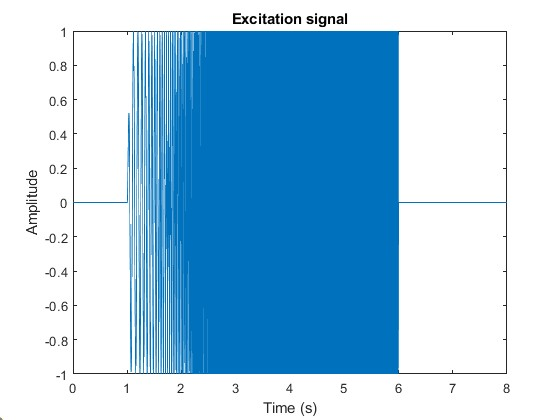
\includegraphics[width=\linewidth]{imagenes/ExcitationSignal_RIR_Measurement.jpg}
        \caption{\footnotesize Señal de excitación (Barrido senoidal)}
        \label{fig:sub1}
    \end{subfigure}
    \hfill
    \begin{subfigure}{0.3\textwidth}
        \centering
        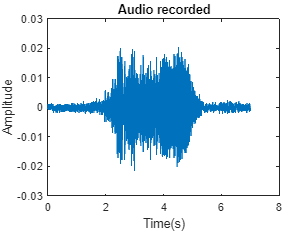
\includegraphics[width=\linewidth]{imagenes/AudioFromDevice_RIR_Measurement.png}
        \caption{\footnotesize Audio grabado}
        \label{fig:sub2}
    \end{subfigure}
    \hfill
    \begin{subfigure}{0.3\textwidth}
        \centering
        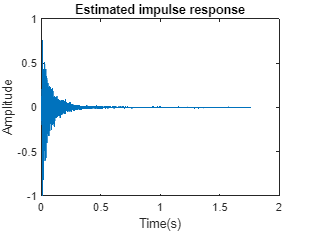
\includegraphics[width=\linewidth]{imagenes/EstimatedImpulseResponse_RIR_Measurement.png}
        \caption{\footnotesize Respuesta al impulso estimada}
        \label{fig:sub2}
    \end{subfigure}
    \caption{Gráficas resultantes de generación y medición de la acústica}
\end{figure}
\FloatBarrier

El programa completo se encuentra como () en el Anexo ().

\subsubsection{MF1.1. Procesamiento de la respuesta y calculo de la acústica}
A partir de la respuesta al impulso de un recinto, se pueden derivar distintos parámetros acústicos, como los establecidos en la \href{https://www.iso.org/standard/36201.html}{ISO-3382}. Siendo que la respuesta al impulso la podemos obtener de mediciones físicas, de simulaciones del recinto, e incluso de bancos de datos con respuestas de múltiples recintos para fines de validación, fue necesario tener una metodología general que nos permitiera analizar datos de diferentes fuentes. \hfill\break
El programa de generación y medición de la acústica, tiene como salida una estructura con los datos de la respuesta al impulso y el tiempo de muestreo; para las simulaciones y los bancos de datos, las respuestas al impulso se guardan como un archivo de tipo \textit{wav}. Se iniciara con una linea de lectura de archivos de este tipo, que se desactivara en caso de usarse consecutivo al programa de generación y medición de la acústica. Dicho código también se encargara de combinar las señales en caso de leer archivos \textit{wav} con múltiples canales.
\begin{lstlisting}[frame=single,numbers=left, style=Matlab-editor, basicstyle=\tiny]
[temp_y,ImpulseResponse.fs] = audioread(['C:\Users\User\Desktop\RIR_Database\' ...
    '382908__uzbazur__little-basement-ir-impulse-response.wav']);
if size(temp_y,2) > 1
    ImpulseResponse.y = mean(temp_y,2);
end
\end{lstlisting}
De acuerdo con la norma ISO-3382, los parámetros acústicos que caracterizan un cuarto son:
\begin{itemize}
    \item $EDT$, tiempo de decaimiento temprano
    \item $T_{20}$ tiempo de reverberación referido a -20 Db
    \item $T_{30}$ tiempo de reverberación referido a -30 Db
    \item $C_{50}$ claridad a 50 ms
    \item $C_{80}$ claridad a 80 ms
    \item $D_{50}$ ratio de energía útil
    \item $G$ fuerza del sonido 
\end{itemize}
Todos los parámetros anteriores, deben calcularse en las frecuencias centrales de las bandas de frecuencia pertenecientes octavas de 125 Hz a 4000 Hz. Por esto, primero se deben pasar por filtros pasa-bandas, distribuidos a lo largo de las octavas.
Se paso la respuesta al impulso por 6 filtros, con frecuencias centrales y rangos como se muestra a continuación \href{https://www.doctorproaudio.com/content.php?2402-octaves-and-third-octaves#:~:text=As%20a%20reference%2C%20the%20central,exactly%20to%20double%20or%20half.}{Fuente}:
\begin{center}
    \begin{longtable}[!htb]{ |c|c|c| }
    \hline
    Frecuencia central & Limite inferior & Limite superior \\ 
    \hline
    125 Hz & 88.39 Hz & 176.8 Hz   \\  
    250 Hz & 176.8 Hz & 353,6 Hz   \\  
    500 Hz & 353.6 Hz & 707.1 Hz   \\  
    1000 Hz & 707.1 Hz & 1414 Hz   \\  
    2000 Hz & 1414 Hz & 2828 Hz     \\  
    4000 Hz & 2828 Hz & 5657 HZ   \\
    \hline
    \caption{Rangos de frecuencias para filtros}
    \label{tab:Rangos De Frecuencias}
    \end{longtable} 
\end{center}
\begin{lstlisting}[frame=single,numbers=left, style=Matlab-editor, basicstyle=\tiny]
RIR = struct('General',ImpulseResponse); 
RIR.f125.y = bandpass(ImpulseResponse.y,[88.39 176.8],ImpulseResponse.fs);
RIR.f125.fs = ImpulseResponse.fs;
RIR.f250.y = bandpass(ImpulseResponse.y,[176.8 353.6],ImpulseResponse.fs);
RIR.f250.fs = ImpulseResponse.fs;
RIR.f500.y = bandpass(ImpulseResponse.y,[353.6 707.1],ImpulseResponse.fs);
RIR.f500.fs = ImpulseResponse.fs;
RIR.f1k.y = bandpass(ImpulseResponse.y,[707.1 1414],ImpulseResponse.fs);
RIR.f1k.fs = ImpulseResponse.fs;
RIR.f2k.y = bandpass(ImpulseResponse.y,[1414 2828],ImpulseResponse.fs);
RIR.f2k.fs = ImpulseResponse.fs;
RIR.f4k.y = bandpass(ImpulseResponse.y,[2828 5657],ImpulseResponse.fs);
RIR.f4k.fs = ImpulseResponse.fs;
\end{lstlisting}
Se pueden observar algunas la respuesta del recinto para ciertas frecuencias.
\begin{figure}[!htb]
    \centering
     \begin{subfigure}{0.3\textwidth}
        \centering
        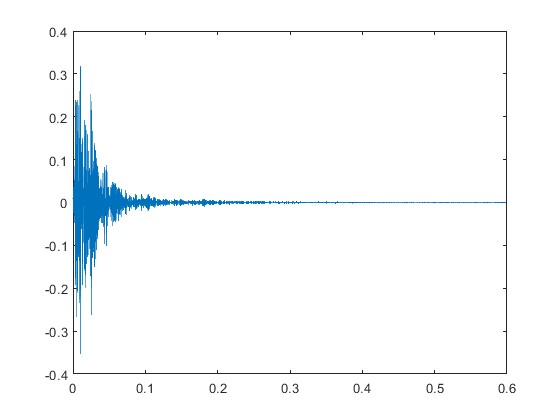
\includegraphics[width=\linewidth]{imagenes/RIR_500Hz_RIR_Measurement.jpg}
        \caption{\footnotesize Respuesta al impulso a 500 Hz}
        \label{fig:sub1}
    \end{subfigure}
    \hfill
    \begin{subfigure}{0.3\textwidth}
        \centering
        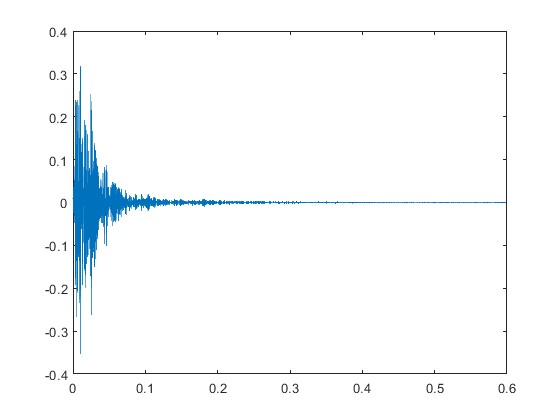
\includegraphics[width=\linewidth]{imagenes/RIR_1000Hz_RIR_Measurement.jpg}
        \caption{\footnotesize Respuesta al impulso a 1000 Hz}
        \label{fig:sub2}
    \end{subfigure}
    \hfill
    \begin{subfigure}{0.3\textwidth}
        \centering
        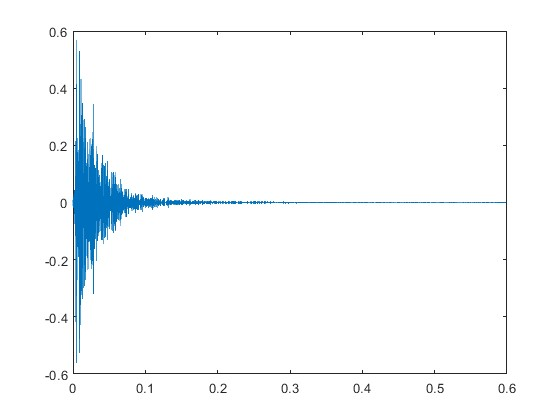
\includegraphics[width=\linewidth]{imagenes/RIR_2000Hz_RIR_Measurement.jpg}
        \caption{\footnotesize Respuesta al impulso a 2000 Hz}
        \label{fig:sub2}
    \end{subfigure}
    \caption{Respuesta al impulso para diferentes frecuencias}
\end{figure}
\FloatBarrier

A continuación podemos hacer el análisis de la respuesta al impulso en sus diferentes frecuencias, además de la general, lo que nos dará los parámetros acústicos actuales del recinto. Este proceso se hace mediante otro \textit{script} llamado \textbf{$RIR\_Analysis$}.\hfill\break
La función toma como primera entrada el método de empaquetado de la señal, se debe ingresar un 1 en caso de que se quiera analizar un archivo de tipo \textit{wav}, y cualquier otro numero en caso de que la señal ya venga empaquetada en una estructura con el tiempo de muestreo y la amplitud. A continuación se introduce la señal correspondiente, además de las dimensiones del cuarto en el que se grabo la respuesta al impulso y una variable booleana que indica al programa si debe mostrar la gráfica de decaimiento de la energía junto con los ajustes lineales y los parámetros.
La función retorna la respuesta al impulso cuadrada, la gráfica de decaimiento, el vector de tiempo correspondiente y una estructura con los parámetros acústicos.

\begin{lstlisting}[frame=single,numbers=left, style=Matlab-editor, basicstyle=\tiny]
function [RIRsq,DC,t,AcousticParams] = RIR_Analisys(method, input, room_dimensions,printFlag)
\end{lstlisting}
La gráfica del decaimiento se obtiene mediante la integral de Schroeder, la cual es una integración hacia atrás, que se hace desde un punto donde la señal ya solo contiene ruido de fondo. \href{https://www.roomeqwizard.com/help/help_en-GB/html/graph_filteredir.html}{Fuentes}
\begin{lstlisting}[frame=single,numbers=left, style=Matlab-editor, basicstyle=\tiny]
    RIRsq = y.^2;
    schroeder_cumsum = cumsum(flipud(RIRsq));
    schroeder_normalized = schroeder_cumsum / max(schroeder_cumsum);
    DC = flipud(10*log10(schroeder_normalized));
\end{lstlisting}
La gráfica se muestra en decibelios y va de 0 a $-\infty$.

\newpage

\rule{\linewidth}{0.4pt}
La curva de decaimiento de la energía nos permite ver el decaimiento exponencial del sonido como un decaimiento lineal, y así, poder ajustar rectas que se apeguen mas al decaimiento de la señal sin verse interferida por el ruido de fondo. Adicionalmente, podemos usar esta curva para calcular los otros parámetros acústicos como $D_{50}$ o $C_{50}$.\hfill\break
\begin{figure}[!htb]
    \centering
    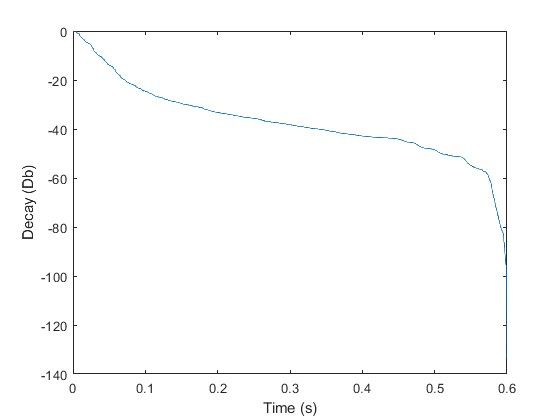
\includegraphics[width=\linewidth]{imagenes/DecayCurve_RIR_Analysis.jpg}
    \caption{\footnotesize Curva de decaimiento}
    \label{fig:DecayCurve}
\end{figure}
\FloatBarrier
El comportamiento de la curva deja de ser lineal cuando la señal comienza a verse afectada por el ruido de fondo. Idealmente, el ruido de fondo debería presentarse como un valle horizontal, y la señal con un decaimiento lo mas recto posible, hasta curvarse al final para convertirse en el valle del ruido de fondo. \hfill\break
El análisis de esta curva revela la importancia de tener una excitación lo bastante fuerte como para superar al ruido de fondo y ver el decaimiento de la curva por mas tiempo antes de comenzar a perder información. Es por esto también que, a pesar de que el tiempo de reverberación esta referido a -60 Db, no suele medirse el decaimiento de esta manera, si no que se recurre a medir un decaimiento de -20 Db o -30 Db y se hace una extrapolación hasta los -60 Db. La norma ISO-3382 recomienda comenzar a medir el decaimiento hasta los -5 Db, para evitar interferencias de armónicos y entonces disminuir 20 o 30 Db. Intentar observar el decaimiento hasta -65 Db, implica que para un ruido de fondo de unos 30 Db, requeriríamos excitar el cuarto con una señal de al menos 95 Db, lo cual escapa de las posibilidades dentro de un recinto relativamente pequeño.\hfill\break
Posteriormente, se ajustan rectas tomando en cuenta los intervalos de -20 Db, -30 Db y del EDT.
\begin{lstlisting}[frame=single,numbers=left, style=Matlab-editor, basicstyle=\tiny]
    [~, EDT_Idx1] = min(abs(LF_EDT+10));
    [~, EDT_Idx2] = min(abs(LF_EDT));
    T60delEDT = 6*(t(EDT_Idx1)-t(EDT_Idx2));
    
    [~, EDT_Idx1] = min(abs(LF_T20+20));
    [~, EDT_Idx2] = min(abs(LF_T20));
    T60delT20 = 3*(t(EDT_Idx1)-t(EDT_Idx2));
    
    [~, EDT_Idx1] = min(abs(LF_T30+30));
    [~, EDT_Idx2] = min(abs(LF_T30));
    T60delT30 = 2*(t(EDT_Idx1)-t(EDT_Idx2));
\end{lstlisting}
La relación de energía útil ($D$) se define como la relación entre la energía total y la energía de la señal con arribo temprano. Se utilizan $D_{50}$ y $D_{80}$ para definir este parámetro usando 50 y 80 ms respectivamente como el limite para el arribo temprano. Cabe resaltar que este tiempo se toma a partir del momento que llega la señal directa (en linea recta de la fuente al receptor).
\begin{lstlisting}[frame=single,numbers=left, style=Matlab-editor, basicstyle=\tiny]
    [~,maxIdx] = max(RIRsq);
    RIRsq_trunc = RIRsq(maxIdx:end);
    Energy0_50 = trapz(RIRsq_trunc(1:round(0.05*fs)));
    Energy0_80 = trapz(RIRsq_trunc(1:round(0.08*fs)));
    Energy0_end = trapz(RIRsq_trunc(1:end));
    
    D50 = Energy0_50/Energy0_end;
    D80 = Energy0_80/Energy0_end;
\end{lstlisting}
Los índices de claridad $C_{50}$ y $C_{80}$ siguen la misma definición que el índice $D$, pero, en lugar de representar un ratio o porcentaje, estos se presentan en Db como escala logarítmica. El índice $C_{50}$ se puede entender como la claridad del habla y $C_{80}$ como la claridad de la musica. Ambos se pueden calcular a partir del índice $D$ como:
$$C_{50/80} = 10 log \left( \frac{D_{50/80}}{1-D_{50/80}} \right)$$

\begin{lstlisting}[frame=single,numbers=left, style=Matlab-editor, basicstyle=\tiny]
    C50 = 10*log(D50/(1-D50));
    C80 = 10*log(D80/(1-D80));
\end{lstlisting}

Por ultimo, la fuerza del sonido $G$ se define como la relación entre el nivel de presión del sonido en el recinto y el nivel de presión del mismo sonido en un campo libre, es decir, sin reflexiones, únicamente el sonido directo. \hfill\break
La medición de este parámetro es un poco mas complicada, ya que se requiere aislar de todas las reflexiones, al pico en la amplitud producido por el sonido directo. Por esto, se decidió hacer una estimación validada por \cite{Rossing2007}, que relaciona la fuerza del sonido con el tiempo de reverberación en un recinto y sus dimensiones.
$$G = 10 log_{10}\left(\frac{RT_{60}}{V}\right)$$

El ultimo análisis que se hace a la respuesta al impulso es respecto a los modos de vibración. Un recinto con paredes ortogonales, presenta distancias entre paredes que es un múltiplo de la longitud de onda de distintas frecuencias. Lo anterior ocasiona que las ondas oscilen entre paredes como si estuvieran ancladas a las paredes. Cuando el sonido es persistente o el tiempo de reverberación alto, un oyente puede encontrar que existen zonas del cuarto donde el sonido es muy fuerte y otras donde el sonido es muy bajo y se puede medir el cambio en el volumen si se desplaza por el recinto. \hfill\break
Los modos de vibración pueden ser axiales, tangenciales y oblicuos, dependiendo del numero de superficies en las que rebota. Los modos de vibración axiales suelen ser los mas significativos y por suerte, son los mas fáciles de predecir. \hfill\break
Podemos calcular los modos de vibración calculando las frecuencias en donde las dimensiones del cuarto son múltiplos de sus respectivas longitudes de onda. El programa cuenta con un \textit{script} externo llamado \textbf{CalcRoomModes} que realiza esta operación. El programa retorna los primeros n modos axiales de vibración.
\begin{lstlisting}[frame=single,numbers=left, style=Matlab-editor, basicstyle=\tiny]
    c = 343; % m/s
    f_length = c/room_dim(1);
    f_width = c/room_dim(2);
    f_depth = c/room_dim(3);
    modes_length = zeros(1,num_modes);
    modes_width = zeros(1,num_modes);
    modes_depth = zeros(1,num_modes);

    for i = 1:num_modes
        modes_length(i) = f_length*(0.5*i); 
        modes_width(i) = f_width*(0.5*i);
        modes_depth(i) = f_depth*(0.5*i);
    end
\end{lstlisting}
Adicionalmente, el programa se encarga de calcular la frecuencia de Schroeder, la cual nos indica la frecuencia a la que el sonido dentro de un recinto deja de estar dominado por los modos de vibración y pasa a comportarse como un campo difuso. Se calcula con la siguiente formula:
$$f_s = 2000\sqrt{\frac{RT_{60}}{V}}$$
El calculo de este parámetro es importante, debido a que el resto de parámetros acústicos solo son validos si el sonido presente en el recinto se comporta mayormente como un campo difuso. Como se ve en la formula, la variable libre de la que depende esta frecuencia es el tiempo de reverberación; esto nos ayudara a introducir cotas para el tiempo de reverberación que nos asegure no tener modos de vibración significativos durante la reproducción de musica en el estudio.
La ecuación de Sabine (cita) relaciona el tiempo de reverberación con la absorción de las superficies del cuarto y su geometría. 
\begin{displaymath}
    RT_{60} = \frac{0.161 V}{S \alpha}
\end{displaymath}\
Podemos utilizar esta ecuación para tener una relación entre el tiempo de reverberación del cuarto y la superficie de absorción. Debido a que conocemos las absorciones tanto de los paneles como de las paredes, eso deja a la superficie como parámetro libre. Entonces, el control acústico consistirá en encontrar la cantidad de absorción especifica para alcanzar un tiempo de reverberación deseado, y con ella, obtener la cantidad de superficie de paneles acústicos que debemos añadir en el cuarto para alcanzar dicho tiempo de reverberación.
\begin{lstlisting}[frame=single,numbers=left, style=Matlab-editor, basicstyle=\tiny]
    V = prod(room_dim);
    Current_abs = 0.161*V/AcousticParams.General.T60delT20;
    DesiredT60 = 0.27
    Needed_abs = 0.161*V/DesiredT60;
    Offset_abs = Needed_abs-Current_abs;
    MaterialAbs.Abs_Panels = 0.8;
    MaterialAbs.Wall = 0.02;
    Surface = Offset_abs/(MaterialAbs.Abs_Panels-MaterialAbs.Wall)
\end{lstlisting}

%--------------------------------------------------------------------
\paragraph{RayTracingImpulseResponse}\hfill \break
En este programa se simula la respuesta al impulso en una sala con el objetivo de modelar las propiedades reverberantes de un espacio sin tener que realizar mediciones acústicas. La metodología usada presente en \href{http://publications.rwth-aachen.de/record/50580/files/3875.pdf}{Real-Time Auralization}, consiste en tratar el sonido como rayos que viajan en un recinto, los cuales se emiten de manera aleatoria y uniforme, y chocan contra diferentes superficies, perdiendo energía en el proceso. Además, cuando los rayos chocan con una superficie esta refleja los rayos de manera difusa, por lo que una parte de la energía termina en el receptor. La simulación consiste en seguir el camino de los rayos para observar como pierden energía y calcular cuanta energía llega al receptor en cada reflexión, esto para construir un histograma dependiente de la frecuencia y después, obtener la respuesta al impulso pesando un proceso aleatorio de Poisson con el histograma. \\
El programa esta basado en una implementación derivada de \href{https://www.mathworks.com/help/audio/ug/room-impulse-response-simulation-with-stochastic-ray-tracing.html}{\textit{Room Impulse Response Simulation with Stochastic Ray Tracing}}, la cual no nos permite tener caracteristicas localizadas, sino que las toma uniformes en toda la pared, lo cual entre en conflicto con la colocación de paneles acústicos. \\
Para empezar se colocan las dimensiones de la sala, para posteriormente colocar las posiciones del emisor y del receptor y colocar el radio del micrófono, el cual en este caso es de 8.75cm.\\
\begin{figure}[!htb]
    \centering
    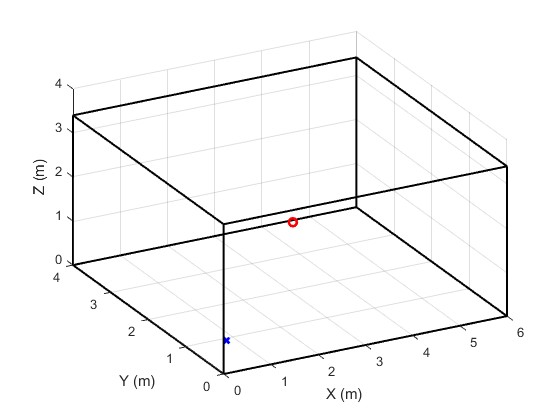
\includegraphics[width=\linewidth]{imagenes/plotRoom.jpg}
    \caption{\footnotesize Geometría del cuarto simulado y posiciones del emisor y receptor}
    \label{fig:plotRoom}
\end{figure}
\FloatBarrier
En la siguiente sección se generan los rayos, los cuales son emanados de la fuente en direcciones aleatorias. Para generar los rayos se utiliza la función RandSampleSphere, dichos rayos son una matriz N por 3 y cada fila de rayos mantiene la dirección del vector de rayos tridimensional.\\
Posteriormente en el código se definen los coeficientes de reflexión y dispersión. Un rayo de sonido se refleja cuando incide sobre una superficie. La reflexión es una combinación de un componente especular y un componente difuso. El coeficiente de absorción es una medida de cuánto sonido se absorbe (en lugar de reflejarse) al golpear una superficie, mientras que el coeficiente de difusión indica que tan especular o difusa es la reflexión.\\
Debido a que los parámetros acústicos se calculan para diferentes bandas de frecuencia, se tiene que hacer un análisis en diferentes frecuencias, dadas por FVect.
\begin{lstlisting}[frame=single,numbers=left, style=Matlab-editor, basicstyle=\tiny]
clear; close all; clc;

%% SetUp
SetUpStruct.room = [10 8 4];
SetUpStruct.src_pos = [2 2 2];
SetUpStruct.mic_pos = [5 5 1.8];
SetUpStruct.mic_radius = 0.0875;
impResTime = 10;

plotRoom(SetUpStruct.room,SetUpStruct.mic_pos,SetUpStruct.src_pos,1)

%% Generate Rays
N = 5000;
rng(0)
rays = RandSampleSphere(N);

%% Reflections and Scattering Coefficients
FVect = [125 250 500 1000 2000 4000];

abs_coeffs = [];
abs_coeffs(:,1) = [0.02,0.02,0.03,0.03,0.04,0.05,0.05]; %Concrete
abs_coeffs(:,2) = [0.70,0.45,0.65,0.60,0.75,0.65,0.65]; %AbsPanels
abs_coeffs(:,3) = [0.14,0.10,0.06,0.08,0.10,0.10,0.10]; %Door

scatt_coeffs = [];
scatt_coeffs(:,1) = [0.30,0.50,0.60,0.60,0.70,0.70,0.70];
scatt_coeffs(:,2) = [0.30,0.50,0.60,0.60,0.70,0.70,0.70];
scatt_coeffs(:,3) =  [0.30,0.50,0.60,0.60,0.70,0.70,0.70];
\end{lstlisting}
A continuación se hace la modificación al programa, creando un mapa de cada una de las paredes, que contiene valores diferentes de absorción y difusión para cada centímetro cuadrado de la pared. 
\begin{lstlisting}[frame=single,numbers=left, style=Matlab-editor, basicstyle=\tiny]
abs_map = {};
abs_map{1} = zeros(round(room_dim(2)*100),round(room_dim(3)*100),num_FBands);
abs_map{2} = zeros(round(room_dim(2)*100),round(room_dim(3)*100),num_FBands);
abs_map{3} = zeros(round(room_dim(1)*100),round(room_dim(3)*100),num_FBands);
abs_map{4} = zeros(round(room_dim(1)*100),round(room_dim(3)*100),num_FBands);
abs_map{5} = zeros(round(room_dim(1)*100),round(room_dim(2)*100),num_FBands);
abs_map{6} = zeros(round(room_dim(1)*100),round(room_dim(2)*100),num_FBands);

scatt_map = {};
scatt_map{1} = zeros(round(room_dim(2)*100),round(room_dim(3)*100),num_FBands);
scatt_map{2} = zeros(round(room_dim(2)*100),round(room_dim(3)*100),num_FBands);
scatt_map{3} = zeros(round(room_dim(1)*100),round(room_dim(3)*100),num_FBands);
scatt_map{4} = zeros(round(room_dim(1)*100),round(room_dim(3)*100),num_FBands);
scatt_map{5} = zeros(round(room_dim(1)*100),round(room_dim(2)*100),num_FBands);
scatt_map{6} = zeros(round(room_dim(1)*100),round(room_dim(2)*100),num_FBands);
\end{lstlisting}
A continuación, la función \textit{updateAbsScattCoefs} nos ayuda a actualizar los mapas de absorción y difusión, colocando los valores de absorción y difusión correspondientes a cada banda de frecuencia, en las índices del mapa correspondientes a sus posiciones en la pared.
\begin{lstlisting}[frame=single,numbers=left, style=Matlab-editor, basicstyle=\tiny]
[abs_map, scatt_map] = updateAbsScattCoeffs(abs_map,scatt_map,1,abs_coeffs(:,1),...
    scatt_coeffs(:,1),[0,0],[room_dim(2),room_dim(3)]); %SmallWall
[abs_map, scatt_map] = updateAbsScattCoeffs(abs_map,scatt_map,2,abs_coeffs(:,1),...
    scatt_coeffs(:,1),[0,0],[room_dim(2),room_dim(3)]); %OpSmallWall
[abs_map, scatt_map] = updateAbsScattCoeffs(abs_map,scatt_map,3,abs_coeffs(:,1),...
    scatt_coeffs(:,1),[0,0],[room_dim(1),room_dim(3)]); %LargeWall
[abs_map, scatt_map] = updateAbsScattCoeffs(abs_map,scatt_map,4,abs_coeffs(:,1),...
    scatt_coeffs(:,1),[0,0],[room_dim(1),room_dim(3)]); %OpLargeWall
[abs_map, scatt_map] = updateAbsScattCoeffs(abs_map,scatt_map,5,abs_coeffs(:,1),...
    scatt_coeffs(:,1),[0,0],[room_dim(1),room_dim(2)]); %Floor
[abs_map, scatt_map] = updateAbsScattCoeffs(abs_map,scatt_map,6,abs_coeffs(:,1),...
    scatt_coeffs(:,1),[0,0],[room_dim(1),room_dim(2)]); %Ceiling
\end{lstlisting}
Como los mapas están vacíos al crearse, primero se definen todas las paredes del cuarto con los respectivos coeficientes de absorción y difusión, y posteriormente ya se pueden actualizar ciertas zonas, con los coeficientes correspondientes a los paneles. \\
El mapa de reflexiones se obtiene a partir del mapa de absorción siguiendo la siguiente \href{https://www.researchgate.net/publication/276288771_Scattering_in_Room_Acoustics_and_Related_Activities_in_ISO_and_AES}{formula}
\begin{displaymath}
    Ref = \sqrt{1-Abs}
\end{displaymath}
\begin{lstlisting}[frame=single,numbers=left, style=Matlab-editor, basicstyle=\tiny]
ref_map = cell(1,num_FBands);
for i = 1:numel(abs_map)
    ref_map{i} = sqrt(1-abs_map{i});
end
\end{lstlisting}
Se definen tambien los parametros del histograma.
\begin{lstlisting}[frame=single,numbers=left, style=Matlab-editor, basicstyle=\tiny]
histTimeStep = 0.0010;
nTBins = round(impResTime/histTimeStep);
nFBins = length(FVect);
TFHist = zeros(nTBins,nFBins);
\end{lstlisting}
El proceso de \textit{Ray-Tracing} comienza tomando un rayo dentro de una banda de frecuencia, tomando su posición, dirección, el tiempo del rayo y su energía, y posteriormente, calcular en donde va a colisionar. Esto se hace observando los signos de la dirección del rayo, los cuales nos dice con cual, de entre dos paredes paralelas, va a colisionar el rayo. A continuación, se calcula el desplazamiento necesario para llegar a la coordenada constante de una pared y resaltando que chocara con la pared para la que necesite el menor desplazamiento. Este calculo se hace dentro de la funcion \textit{GetImpactWall}
\begin{lstlisting}[frame=single,numbers=left, style=Matlab-editor, basicstyle=\tiny]
function [surfaceofimpact,displacement] = getImpactWall(ray_xyz,ray_dxyz,roomDims)
% GETIMPACTWALL Determine which wall the ray encounters
surfaceofimpact = -1;
displacement = 1000;
%  Compute time to intersection with x-surfaces
if (ray_dxyz(1) < 0)
    displacement = -ray_xyz(1) / ray_dxyz(1);
    if displacement==0
        displacement=1000;
    end
    surfaceofimpact = 1; %"SmallWall"
elseif (ray_dxyz(1) > 0)
    displacement = (roomDims(1) - ray_xyz(1)) / ray_dxyz(1);
    if displacement==0
        displacement=1000;c
    end
    surfaceofimpact = 2; %"OpSmallWall"
end
% Compute time to intersection with y-surfaces
if ray_dxyz(2)<0
    t = -ray_xyz(2) / ray_dxyz(2);
    if (t<displacement) && t>0
        surfaceofimpact = 3; %"LargeWall";
        displacement = t;
    end
elseif ray_dxyz(2)>0
    t = (roomDims(2) - ray_xyz(2)) / ray_dxyz(2);
    if (t<displacement) && t>0
        surfaceofimpact =  4; %"OpLargeWall";
        displacement = t;
    end
end
% Compute time to intersection with z-surfaces
if ray_dxyz(3)<0
    t = -ray_xyz(3) / ray_dxyz(3);
    if (t<displacement) && t>0
        surfaceofimpact = 5; %"Floor";
        displacement = t;
    end
elseif ray_dxyz(3)>0
    t = (roomDims(3) - ray_xyz(3)) / ray_dxyz(3);
    if (t<displacement) && t>0
        surfaceofimpact = 6; %"Ceiling";
        displacement = t;
    end
end

displacement = displacement * ray_dxyz;

end
\end{lstlisting}
El desplazamiento y la pared de impacto, nos permite obtener las coordenadas en las que choca el rayo y así, consultar nuestro mapa de reflexión y difusión, para calcular el decaimiento de la energía con base en la reflexión y una nueva dirección para el rayo, la cual es combinación de la reflexión especular y la difusa. \\
Adicionalmente, se usa la difusión en ese punto, para calcular que cantidad de la energía restante del rayo va a capturar el receptor, la cual disminuye conforme mas se aleja del vector normal de la pared. \\
Este proceso se repite para la nueva posición, dirección, tiempo y energía del rayo; hasta que se supere el tiempo de simulación o la energía del rayo disminuya hasta ser despreciable.
\begin{lstlisting}[frame=single,numbers=left, style=Matlab-editor, basicstyle=\tiny]
for iBand = 1:nFBins
    fprintf("Calculating rays for band %d\n",iBand)
    % Perform ray tracing independently for each frequency band.
    for iRay = 1:size(rays,1)
        % Select ray direction
        ray = rays(iRay,:);
        % All rays start at the source/transmitter
        ray_xyz = source_pos;
        % Set initial ray direction. This direction changes as the ray is
        % reflected off surfaces.
        ray_dxyz = ray;
        % Initialize ray travel time. Ray tracing is terminated when the
        % travel time exceeds the impulse response length.
        ray_time = 0;
        % Initialize the ray energy to a normalized value of 1.     Energy
        % decreases when the ray hits a surface.
        ray_energy = 1;

        while (ray_time <= impResTime)

            % Determine the surface that the ray encounters
            [surfaceofimpact,displacement] = getImpactWall(ray_xyz,...
                                             ray_dxyz,room_dim);
            
            % Determine the distance traveled by the ray
            distance = sqrt(sum(displacement.^2));

            % Determine the coordinates of the impact point
            impactCoord = ray_xyz+displacement;

            if surfaceofimpact > 4
                pointOfImpact = [impactCoord(1),impactCoord(2)];
            elseif surfaceofimpact < 3
                pointOfImpact = [impactCoord(2),impactCoord(3)];
            else
                pointOfImpact = [impactCoord(1),impactCoord(3)];
            end

            % Update ray location/source
            ray_xyz = impactCoord;

            % Update cumulative ray travel time
            c = 343; % speed of light (m/s)
            ray_time = ray_time+distance/c;

            % Apply surface reflection to ray's energy
            % This is the amount of energy that is not lost through
            % absorption.

            ReflectionAtPoint = ref_map{surfaceofimpact}(ceil(100*pointOfImpact(1)),ceil(100*pointOfImpact(2)),iBand);
            ray_energy = ray_energy*ReflectionAtPoint;

            % Apply diffuse reflection to ray energy
            % This is the fraction of energy used to determine what is
            % detected at the receiver
            DifussionAtPoint = scatt_map{surfaceofimpact}(ceil(100*pointOfImpact(1)),ceil(100*pointOfImpact(2)),iBand);
            rayrecv_energy = ray_energy*DifussionAtPoint;

            % Determine impact point-to-receiver direction.
            rayrecvvector = mic_pos-impactCoord;

            % Determine the ray's time of arrival at receiver.
            distance = sqrt(sum(rayrecvvector.*rayrecvvector));
            recv_timeofarrival = ray_time+distance/c;

            if recv_timeofarrival>impResTime
                break
            end

            if ray_energy < 0.000001
                break
            end

            % Determine amount of diffuse energy that reaches the receiver.
            % See (5.20) in [2].

            % Compute received energy
            N = getWallNormalVector(surfaceofimpact);
            cosTheta = sum(rayrecvvector.*N)/(sqrt(sum(rayrecvvector.^2)));
            cosAlpha = sqrt(sum(rayrecvvector.^2)-mic_radius^2)/sum(rayrecvvector.^2);
            E = (1-cosAlpha)*2*cosTheta*rayrecv_energy;

            % Update energy histogram
            tbin = floor(recv_timeofarrival/histTimeStep + 0.5);
            TFHist(tbin,iBand) = TFHist(tbin,iBand) + E;

            % Compute a new direction for the ray.
            % Pick a random direction that is in the hemisphere of the
            % normal to the impact surface.
            d = rand(1,3);
            d = d/norm(d);
            if sum(d.*N)<0
                d = -d;
            end

            % Derive the specular reflection with respect to the incident
            % wall
            ref = ray_dxyz-2*(sum(ray_dxyz.*N))*N;

            % Combine the specular and random components
            d = d/norm(d);
            ref = ref/norm(ref);
            ray_dxyz = DifussionAtPoint*d+(1-DifussionAtPoint)*ref;
            ray_dxyz = ray_dxyz/norm(ray_dxyz);
        end
    end
end
\end{lstlisting}
Este proceso nos deja con un histograma dependiente de la frecuencia, el cual representa la envoltura de la respuesta al impulso.
\begin{figure}[!htb]
    \centering
    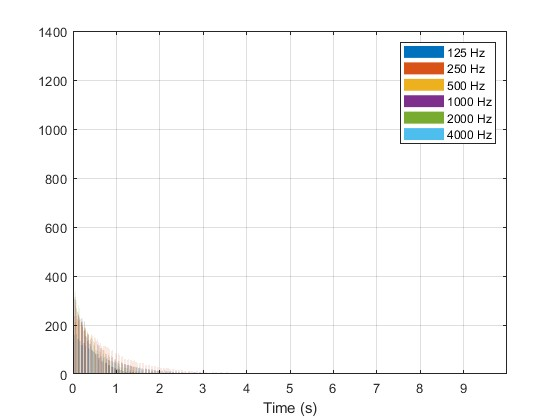
\includegraphics[width=\linewidth]{imagenes/Histogram.jpg}
    \caption{\footnotesize Histograma dependiente de la frecuencia}
    \label{fig:Histograma}
\end{figure}
\FloatBarrier
Para la construcción de la respuesta al impulso, es necesario modelar la estructura detallada a partir del histograma. Esto se puede hacer mediante ruido aleatorio con una distribución de Poisson, y se construye tomando la reflexión de un rayo como evento.\\
Es importante pasar el proceso aleatorio de Poisson por filtros pasa bandas que empaten con las frecuencias del histograma, para asi, poder multiplicarlos. 
\begin{figure}[!htb]
    \centering
    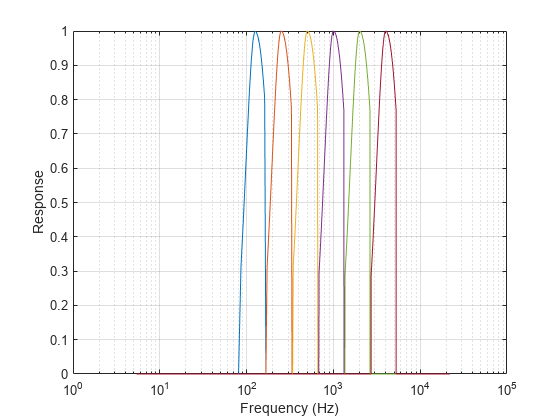
\includegraphics[width=\linewidth]{imagenes/BandPassFilters.png}
    \caption{\footnotesize Filtros pasa-bandas para el proceso de Poisson}
    \label{fig:PoissonFilters}
\end{figure}
\FloatBarrier
\begin{lstlisting}[frame=single,numbers=left, style=Matlab-editor, basicstyle=\tiny]
fs = 44100;
V = prod(room_dim);
t0 = ((2*V*log(2))/(4*pi*c^3))^(1/3); % eq 5.45 in [2]
poissonProcess = [];
timeValues = [];
t = t0;
while (t<impResTime)
    timeValues = [timeValues t]; %#ok
    % Determine polarity.
    if (round(t*fs)-t*fs) < 0 
        poissonProcess = [poissonProcess 1]; %#ok
    else
        poissonProcess = [poissonProcess -1];%#ok
    end
    % Determine the mean event occurence (eq 5.44 in [2])
    mu = min(1e4,4*pi*c^3*t^2/V); 
    % Determine the interval size (eq. 5.44 in [2])
    deltaTA = (1/mu)*log(1/rand); % eq. 5.43 in [2])
    t = t+deltaTA;
end
randSeq = zeros(ceil(impResTime*fs),1);
for index=1:length(timeValues)
    randSeq(round(timeValues(index)*fs)) = poissonProcess(index);
end
flow = [115 225 450 900 1800 3600 7200];
fhigh = [135 275 550 1100 2200 4400 8800];
NFFT = 8192;
win = hann(882,"symmetric");
sfft = dsp.STFT(Window = win,OverlapLength=441,FFTLength=NFFT,FrequencyRange="onesided");
isfft = dsp.ISTFT(Window=win,OverlapLength=441,FrequencyRange="onesided");
F = sfft.getFrequencyVector(fs);
RCF = zeros(length(FVect),length(F));
for index0 = 1:length(FVect)
    for index=1:length(F)
        f = F(index);
        if f<FVect(index0) && f>=flow(index0)
            RCF(index0,index) = .5*(1+cos(2*pi*f/FVect(index0)));
        end
        if f<fhigh(index0) && f>=FVect(index0)
            RCF(index0,index) = .5*(1-cos(2*pi*f/(FVect(index0)+1)));
        end
    end
end
frameLength = 441;
numFrames = length(randSeq)/frameLength;
y = zeros(length(randSeq),numel(FVect));
for index=1:numFrames
    x = randSeq((index-1)*frameLength+1:index*frameLength);
    X = sfft(x);    
    X = X.*RCF.';
    y((index-1)*frameLength+1:index*frameLength,:) = isfft(X);
end
impTimes = (1/fs)*(0:size(y,1)-1);
hisTimes = histTimeStep/2 + histTimeStep*(0:nTBins);
W = zeros(size(impTimes,2),numel(FVect));
BW = fhigh-flow;
for k=1:size(TFHist,1)
    gk0 = floor((k-1)*fs*histTimeStep)+1;
    gk1 = floor(k*fs*histTimeStep);
    yy = y(gk0:gk1,:).^2;
    val = sqrt(TFHist(k,:)./sum(yy,1)).*sqrt(BW/(fs/2));
    for iRay=gk0:gk1
        W(iRay,:)= val;
    end
end
\end{lstlisting}
Por ultimo, podemos crear la respuesta al impulso con los pesos y el histograma. Es importante notar que se agrego ruido de fondo, que nos permita observar el decaimiento en la integral de Schroeder.
\begin{lstlisting}[frame=single,numbers=left, style=Matlab-editor, basicstyle=\tiny]
y_2 = y.*W;
ip = sum(y_2,2);
ip = ip./max(abs(ip));
ip = ip + rand(length(ip),1)/1000;
vectorTiempo = (1/fs)*(0:numel(ip)-1);
figure
plot(vectorTiempo,ip.^2)
grid on
xlabel("Time (s)")
ylabel("Impulse Response")
\end{lstlisting}
\begin{figure}[!htb]
    \centering
    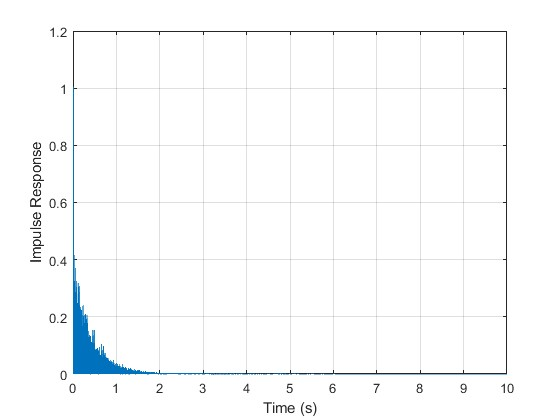
\includegraphics[width=\linewidth]{imagenes/RIRsquared_Simulated.jpg}
    \caption{\footnotesize RIR cuadrada obtenida de simulación}
    \label{fig:RIRsqSimulated}
\end{figure}
\FloatBarrier
A esta respuesta al impulso podemos aplicarle los mismos análisis que hacíamos con una respuesta al impulso obtenida mediante una medición.
\begin{figure}[!htb]
    \centering
    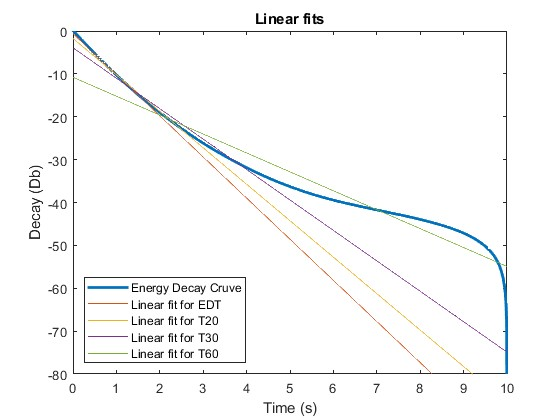
\includegraphics[width=\linewidth]{imagenes/RIRSimulated_Analysis.jpg}
    \caption{\footnotesize Análisis de la respuesta al impulso simulada}
    \label{fig:RIRSimulated_Analysis}
\end{figure}
\FloatBarrier
%------------------------------------------------------------------------------------------
Para comprobar el funcionamiento de nuestra simulación, recurrimos al uso de una paquetería de Python llamada PyRoomAcoustics, la cual permite hacer la simulación tal como la hicimos en MATLAB, pero de manera mas eficiente y con métodos mas completos. Sin profundizar en el funcionamiento, se creo un cuarto igual al de la implementación de MATLAB y se simulo la respuesta al impulso (Se adjunta el codigo utilizado en Anexo ?).
\begin{figure}[!htb]
    \centering
     \begin{subfigure}{0.3\textwidth}
        \centering
        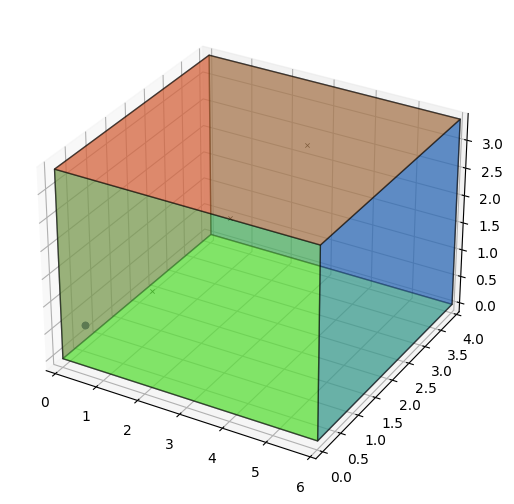
\includegraphics[width=\linewidth]{imagenes/PyRoom_Room.png}
        \caption{\footnotesize Cuarto simulado en PyRoomAcoustics}
        \label{fig:sub2_1}
    \end{subfigure}
    \hfill
    \begin{subfigure}{0.3\textwidth}
        \centering
        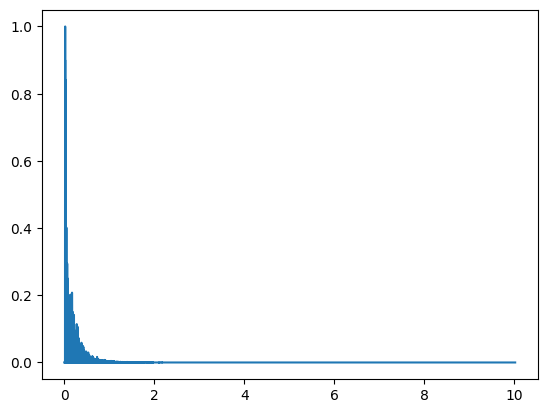
\includegraphics[width=\linewidth]{imagenes/PyRoom_RIR.png}
        \caption{\footnotesize Respuesta al impulso en PyRoomAcoustics}
        \label{fig:sub2_2}
    \end{subfigure}
    \hfill
    \begin{subfigure}{0.3\textwidth}
        \centering
        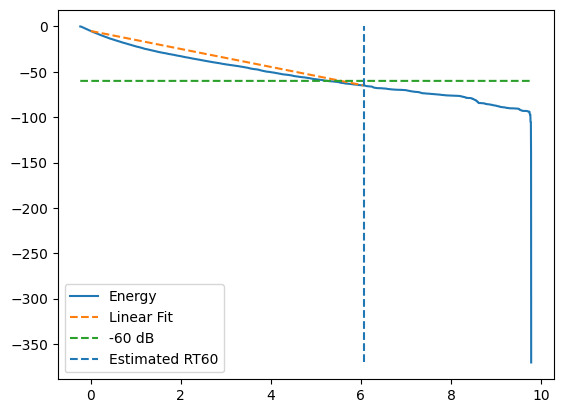
\includegraphics[width=\linewidth]{imagenes/PyRoom_Decay.png}
        \caption{\footnotesize Análisis de la respuesta al impulso en PyRoomAcoustics}
        \label{fig:sub2_3}
    \end{subfigure}
    \caption{Simulación con PyRoomAcoustics}
\end{figure}
\FloatBarrier
Como se puede observar, la simulación en Python arroja resultados muy similares a los obtenidos con la implementación en MATLAB. En el caso de MATLAB, el tiempo de reverberación calculado fue de $6.19 segundos$ mientras que en Python fue de $6.024 segundos$, un tiempo muy cercado considerando que se pierde resolución conforme aumenta el tiempo de reverberación debido a la naturaleza exponencial del decaimiento. \\
Una vez comprobada la implementación en MATLAB, podemos utilizarla con características localizadas de los materiales en las paredes. La simulación aun no es capaz de generar la respuesta al impulso de un recinto lleno (de instrumentos, muebles, decoración, etc.) debido a la complejidad de las interacciones. Para este propósito se buscara la utilización de un software especializado llamado CADNAR.
%------------------------------------------------------------------------

%---------------MF4-----------------------------
\subsubsection{MF3. Módulo modificador de la acústica}
Para realizar la modificación de la acústica en el estudio se debe de cambiar la superficie que interactúa con las ondas de sonido generadas, para poder realizar el cambio de las superficies debemos de girar los prismas triangulares de nuestro trabajo terminal, para lo cual debemos de trasmitir dicho movimiento desde un motor hasta dichos primas. Existen varias formas de transmitir dichos movimiento, en la Tabla \ref{tab:ComTransmision} se pueden 
%-----------------------------tabla-----------------------------
\begin{center}
\footnotesize
    \begin{longtable}[!htb]{| m{5em} | m{12em} | m{12em}| m{12em}|}
    \hline
    \textbf{Tipo}& \textbf{Descripción} & \textbf{Ventajas} & \textbf{Desventajas}\\
    \hline\hline
%---------------------------
    Bandas y poleas& Utilizar poleas y bandas dentadas para poder realizar el movimiento giratorio de los primas triangulares &
    \begin{itemize}
        \item Ruido mínimo
        \item Vibraciones mínimas
        \item Movimiento preciso con una sincronización exacta
        \item Resistencia a la abrasión, al óxido, productos químicos y contaminantes.
    \end{itemize}
    & 
    \begin{itemize}
        \item Se necesitan bandas de largas dimensiones
        \item Mayor costo
        \item Ideal para transferir a una potencia relativamente baja
        \item La potencia de transferencia está a una distancia relativamente menor en comparación con otras bandas de transmisión
    \end{itemize}\\
    \hline
%------------------------
    Tornillo sin fin y corona & Utilizar un tornillo sin fin que mueva coronas, las cuales están acopladas a los primas triangulares &
    \begin{itemize}
        \item Elevada capacidad de carga
        \item Ruido mínimo
        \item Movimiento preciso con una sincronización exacta
        \item Compacto
    \end{itemize}
    & 
    \begin{itemize}
        \item Bajo rendimiento en las etapas de reducción
        \item Requiere mantenimiento periódico debido a que sufren desgaste por fricción
        \item Costo de mantenimiento elevado si se llegara a requerir reparaciones.
    \end{itemize}\\
    \hline
%------------------------    
    Movimiento individual& Colocar un motor por cada uno de los prismas triangulares para controlarlos individualmente& 
    \begin{itemize}
        \item Control personalizado a cada prisma sin la necesidad de ningún otro mecanismo 
        \item Movimiento preciso con una sincronización exacta
    \end{itemize}
    & 
    \begin{itemize}
        \item Elevado costo debido a que se necesitan comprar una gran cantidad de motores
        \item Mayor consumo energético comparado con las otras opciones.
    \end{itemize}\\
    \hline
    \caption{Ventajas y desventajas de los distintos tipos de transmisi\'on de movimiento}
    \label{tab:ComTransmision}
    \end{longtable}
\end{center}

Después de observar las ventajas y desventajas de cada uno de los métodos de transmisión de movimiento nos decidimos por la trasmisión por medio de un tornillo sin fin y corona debido a que se tiene un buen control de la posición de los prismas que portan los paneles, tiene una gran capacidad de carga, además de que el ruido producido es bajo. Al elegir este tipo de transmisión surgieron problemas en cuanto las dimensiones del tornillo sin fin, ya que si optabamos por utilizar un solo tornillo sin fin para mover todos los primas este debia de ser de un largo bastante considerable, y realizar la fabricación de este sería una tarea difícil, por lo que en la Tabla \ref{tab:ComTornilloSF} se comparan las opciones que se tienen para realizar la transmisión de tornillo sin fin y corona.
%-----------------------------tabla-----------------------------
\begin{center}
\footnotesize
    \begin{longtable}[!htb]{| m{5em} | m{12em} | m{12em}| m{12em}|}
    \hline
    \textbf{Tipo}& \textbf{Descripción} & \textbf{Ventajas} & \textbf{Desventajas}\\
    \hline\hline
%---------------------------
    Bandas y poleas& Utilizar poleas y bandas dentadas para poder realizar el movimiento giratorio de los primas triangulares &
    \begin{itemize}
        \item Ruido mínimo
        \item Vibraciones mínimas
        \item Movimiento preciso con una sincronización exacta
        \item Resistencia a la abrasión, al óxido, productos químicos y contaminantes.
    \end{itemize}
    & 
    \begin{itemize}
        \item Se necesitan bandas de largas dimensiones
        \item Mayor costo
        \item Ideal para transferir a una potencia relativamente baja
        \item La potencia de transferencia está a una distancia relativamente menor en comparación con otras bandas de transmisión
    \end{itemize}\\
    \hline
%------------------------
    Tornillo sin fin y corona & Utilizar un tornillo sin fin que mueva coronas, las cuales están acopladas a los primas triangulares &
    \begin{itemize}
        \item Elevada capacidad de carga
        \item Ruido mínimo
        \item Movimiento preciso con una sincronización exacta
        \item Compacto
    \end{itemize}
    & 
    \begin{itemize}
        \item Bajo rendimiento en las etapas de reducción
        \item Requiere mantenimiento periódico debido a que sufren desgaste por fricción
        \item Costo de mantenimiento elevado si se llegara a requerir reparaciones.
    \end{itemize}\\
    \hline
%------------------------    
    Movimiento individual& Colocar un motor por cada uno de los prismas triangulares para controlarlos individualmente& 
    \begin{itemize}
        \item Control personalizado a cada prima sin la necesidad de ningún otro mecanismo 
        \item Movimiento preciso con una sincronización exacta
    \end{itemize}
    & 
    \begin{itemize}
        \item Elevado costo debido a que se necesitan comprar una gran cantidad de motores
        \item Mayor consumo energético comparado con las otras opciones.
    \end{itemize}\\
    \hline
    \caption{Ventajas y desventajas relacionadas a la utilización de un tornillo sin fin único o varios segmentos de tornillo sin fin}
    \label{tab:ComTornilloSF}
    \end{longtable}
\end{center}
\subsubsection{MF4. Módulo de interfaz de usuario}

La interfaz de usuario de nuestra aplicación cuenta con un estilo de diseño neumorfista, respondiendo a las tendencias de diseño actuales, lo que genera una seguridad de uso 
para una aplicación moderna de carácter profesional, con una estética atractiva, consistencia visual, pero sobre todo interactividad y enfoque en el funcionamiento, permitiendo 
a los usuarios interactuar con el sistema de manera eficiente. A continuación, se describe el flujo de trabajo de la interfaz de usuario \ref{fig:diagrama_flujo}. \\

\begin{figure}[!htb]
    \centering
    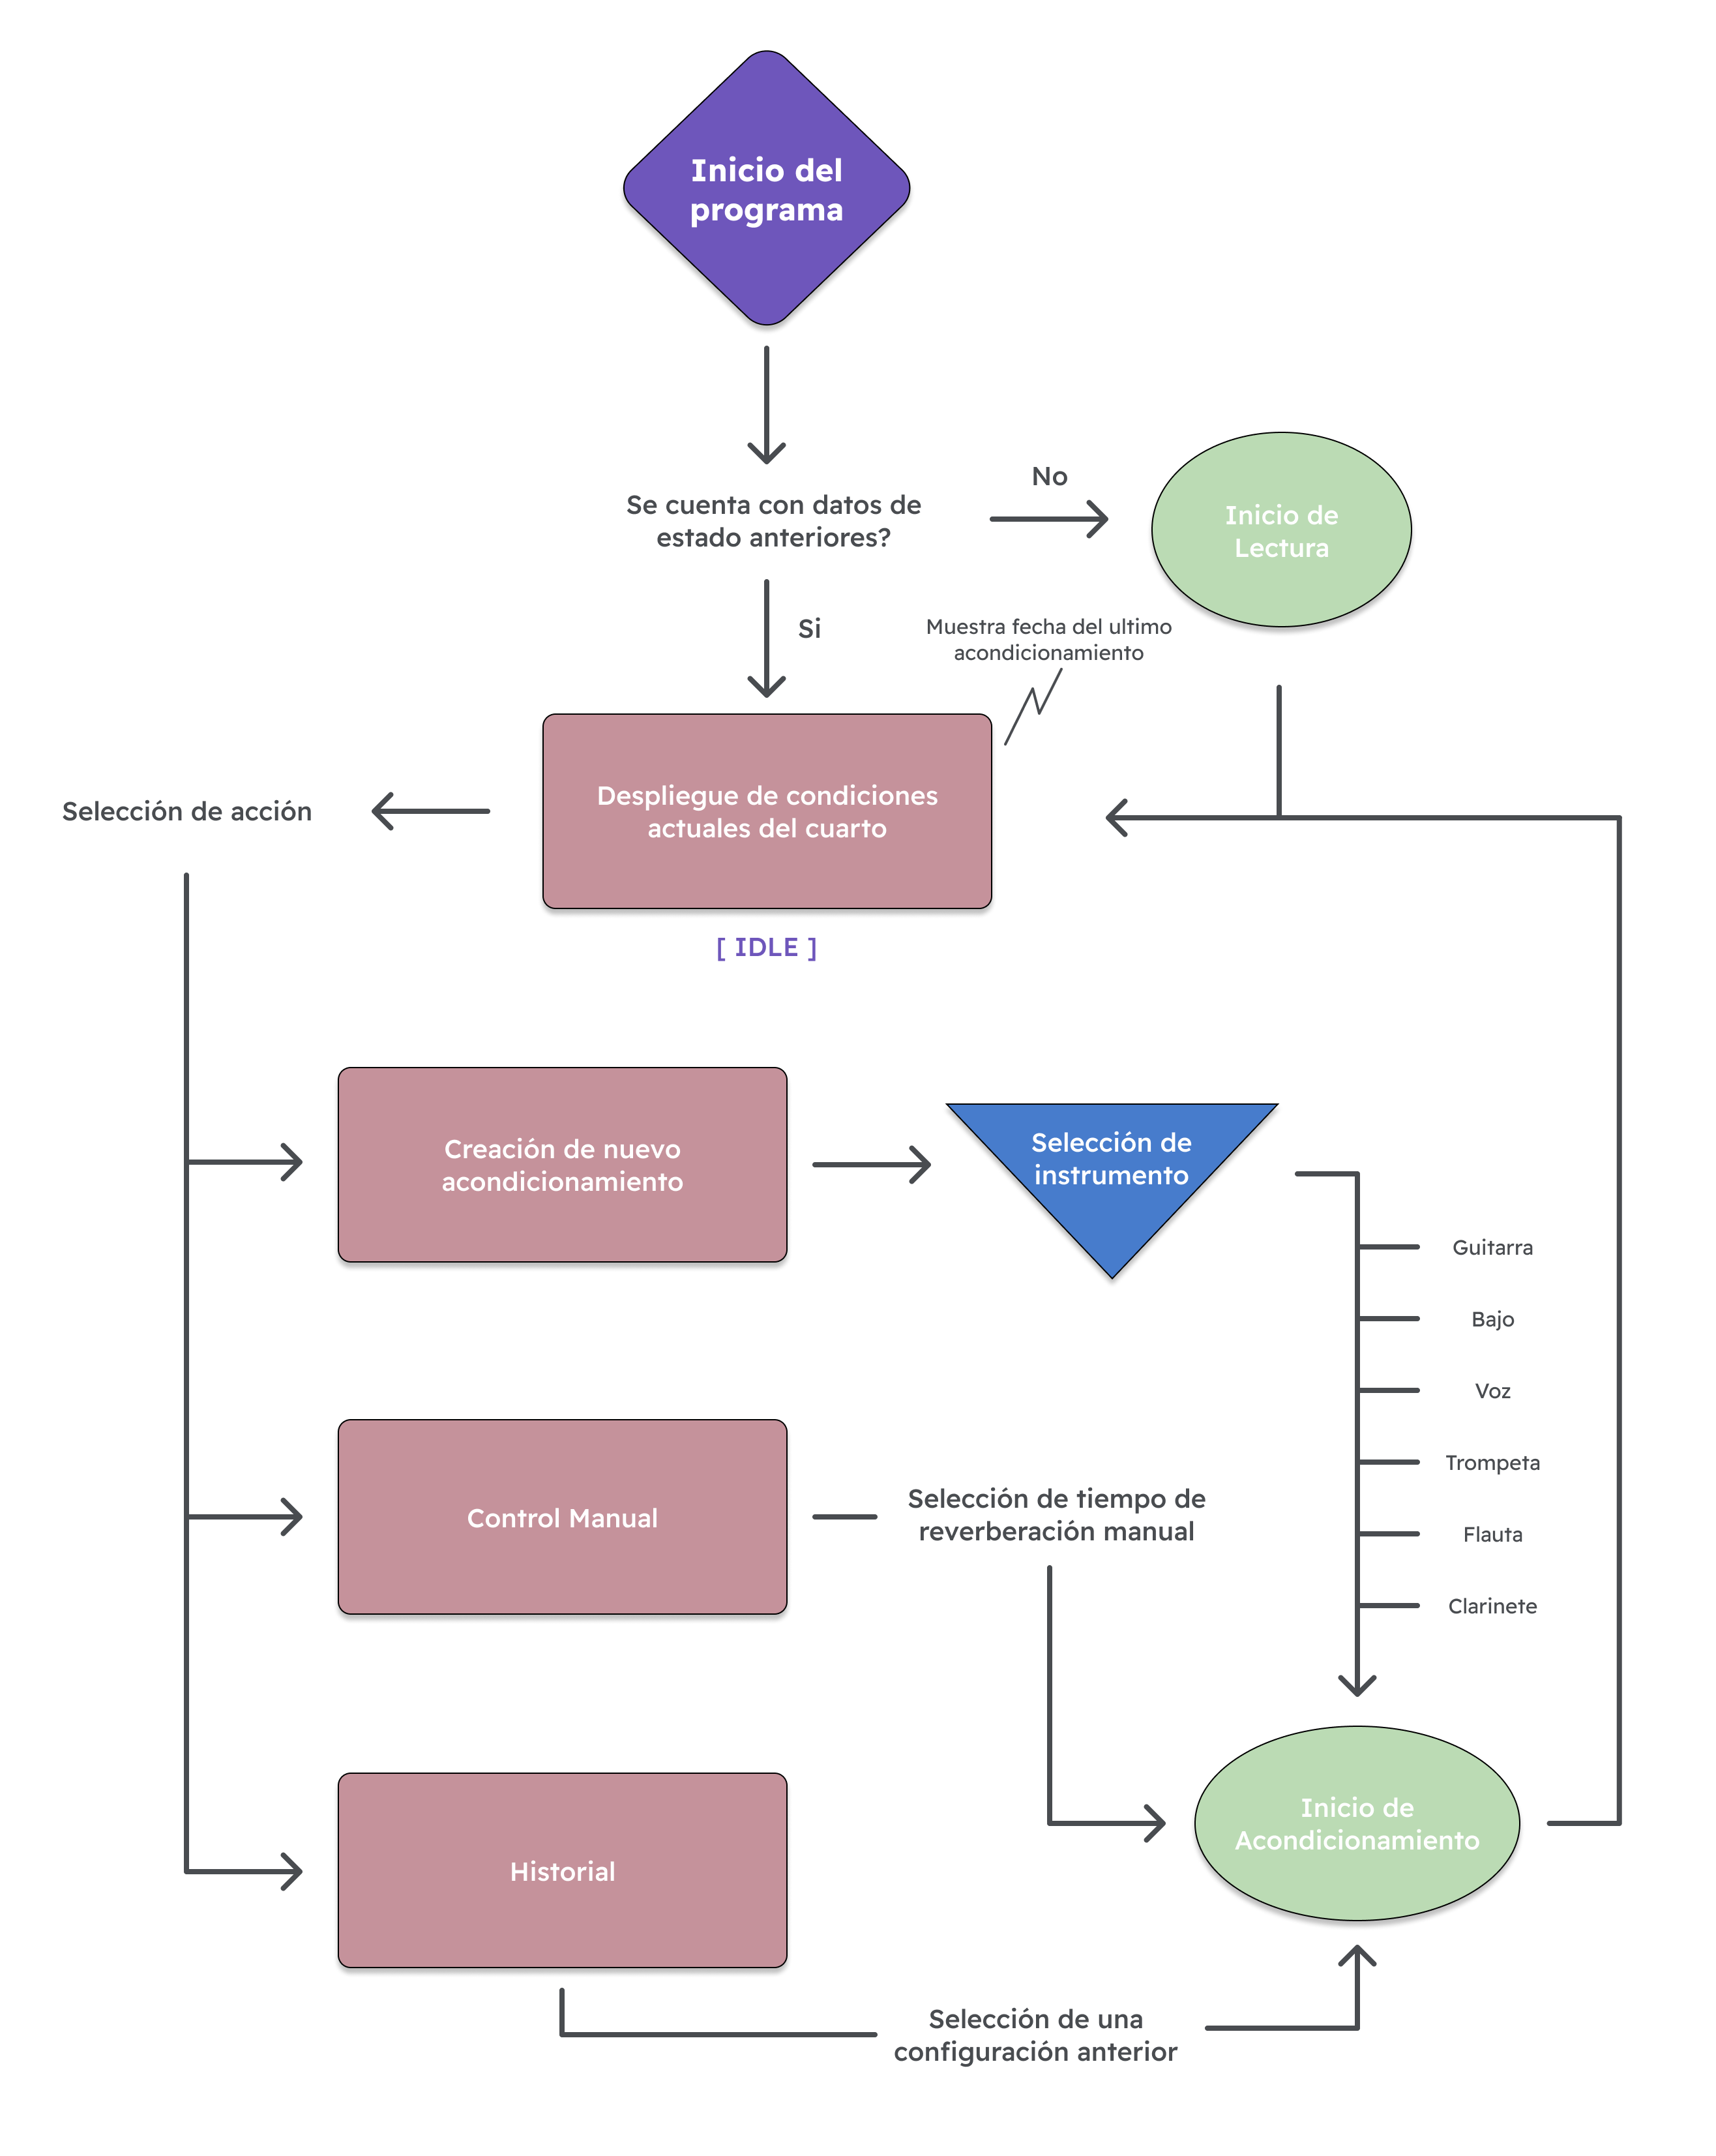
\includegraphics[width=1\linewidth]{imagenes/Diagrama de Flujo.png}
    \caption{Diagrama de Flujo de la aplicación}
    \label{fig:diagrama_flujo}
\end{figure}

Al iniciar el programa, el sistema verifica si hay datos de estado anteriores disponibles para mostrar: \\

\begin{itemize}[label={}, leftmargin=0pt]
    \item \textbf{Inicio del Programa:} El sistema comienza verificando si existen datos de estado previos.
    \item \textbf{Datos de Estado Anteriores:}
    \begin{itemize}
        \item \textbf{Sí:} Si hay datos de estado anteriores, se despliegan las condiciones actuales del cuarto, incluyendo la fecha del último acondicionamiento (MF4.1.).
        \item \textbf{No:} Si no hay datos de estado previos, se inicia el proceso de lectura de datos actuales (MF4.2.). \\
    \end{itemize}
\end{itemize}

Una vez desplegadas las condiciones actuales del cuarto, el sistema se encuentra en estado de reposo, el usuario puede elegir entre las acciones: \\

\begin{itemize}[label={}, leftmargin=0pt]
    \item \textbf{Creación de Nuevo Acondicionamiento:} 
    \begin{itemize}
        \item El usuario selecciona esta opción para iniciar un nuevo acondicionamiento.
        \item \textbf{Selección de Instrumento:} El usuario elige el tipo de instrumento (Guitarra, Bajo, Voz, Trompeta, Flauta, Clarinete).
        \item \textbf{Inicio de Acondicionamiento:} Una vez seleccionado el instrumento, se inicia el acondicionamiento del cuarto.
    \end{itemize}
    \item \textbf{Control Manual:}
    \begin{itemize}
        \item El usuario puede ajustar manualmente el tiempo de reverberación.
        \item \textbf{Inicio de Acondicionamiento:} Después de ajustar manualmente, se procede con el acondicionamiento.
    \end{itemize}
    \item \textbf{Historial:}
    \begin{itemize}
        \item El usuario puede revisar el historial de acondicionamientos previos.
        \item \textbf{Selección de Configuración Anterior:} El usuario puede seleccionar una configuración anterior para replicarla.
        \item \textbf{Inicio de Acondicionamiento:} Una vez seleccionada, se inicia el acondicionamiento. \\
    \end{itemize}
\end{itemize}

La interfaz está compuesta por elementos que facilitan la interacción del usuario con el sistema, estos son: \\

\begin{itemize}[label={}, leftmargin=0pt]
    \item \textbf{Panel de Navegación:} Situado en el lado izquierdo de la pantalla, este panel permite al usuario navegar entre las diferentes secciones de la aplicación, como la visualización de condiciones actuales, la creación de nuevos acondicionamientos, el control manual y el historial.
    \item \textbf{Botón de Iniciar Lectura:} Este botón permite al usuario iniciar la lectura de las condiciones actuales del cuarto en cualquier momento.
    \item \textbf{Estado de Conexión:} Un indicador de conexión muestra si el sistema está conectado correctamente o si ha ocurrido algún fallo.
    \item \textbf{Principal:} Donde se encuentra la información de la diferentes acciones accesibles por el panel de navegación. Es la sección principal de la interfaz y varia su contenido según la pagina en la que se esté ubicado.
\end{itemize}

Finalmente podemos observar las imágenes en la Figura \ref{fig:vistas_interfaz} de las diferentes vistas de la interfaz. \\

\begin{figure}[!htb]
    \centering
    \begin{subfigure}{0.45\textwidth}
        \centering
        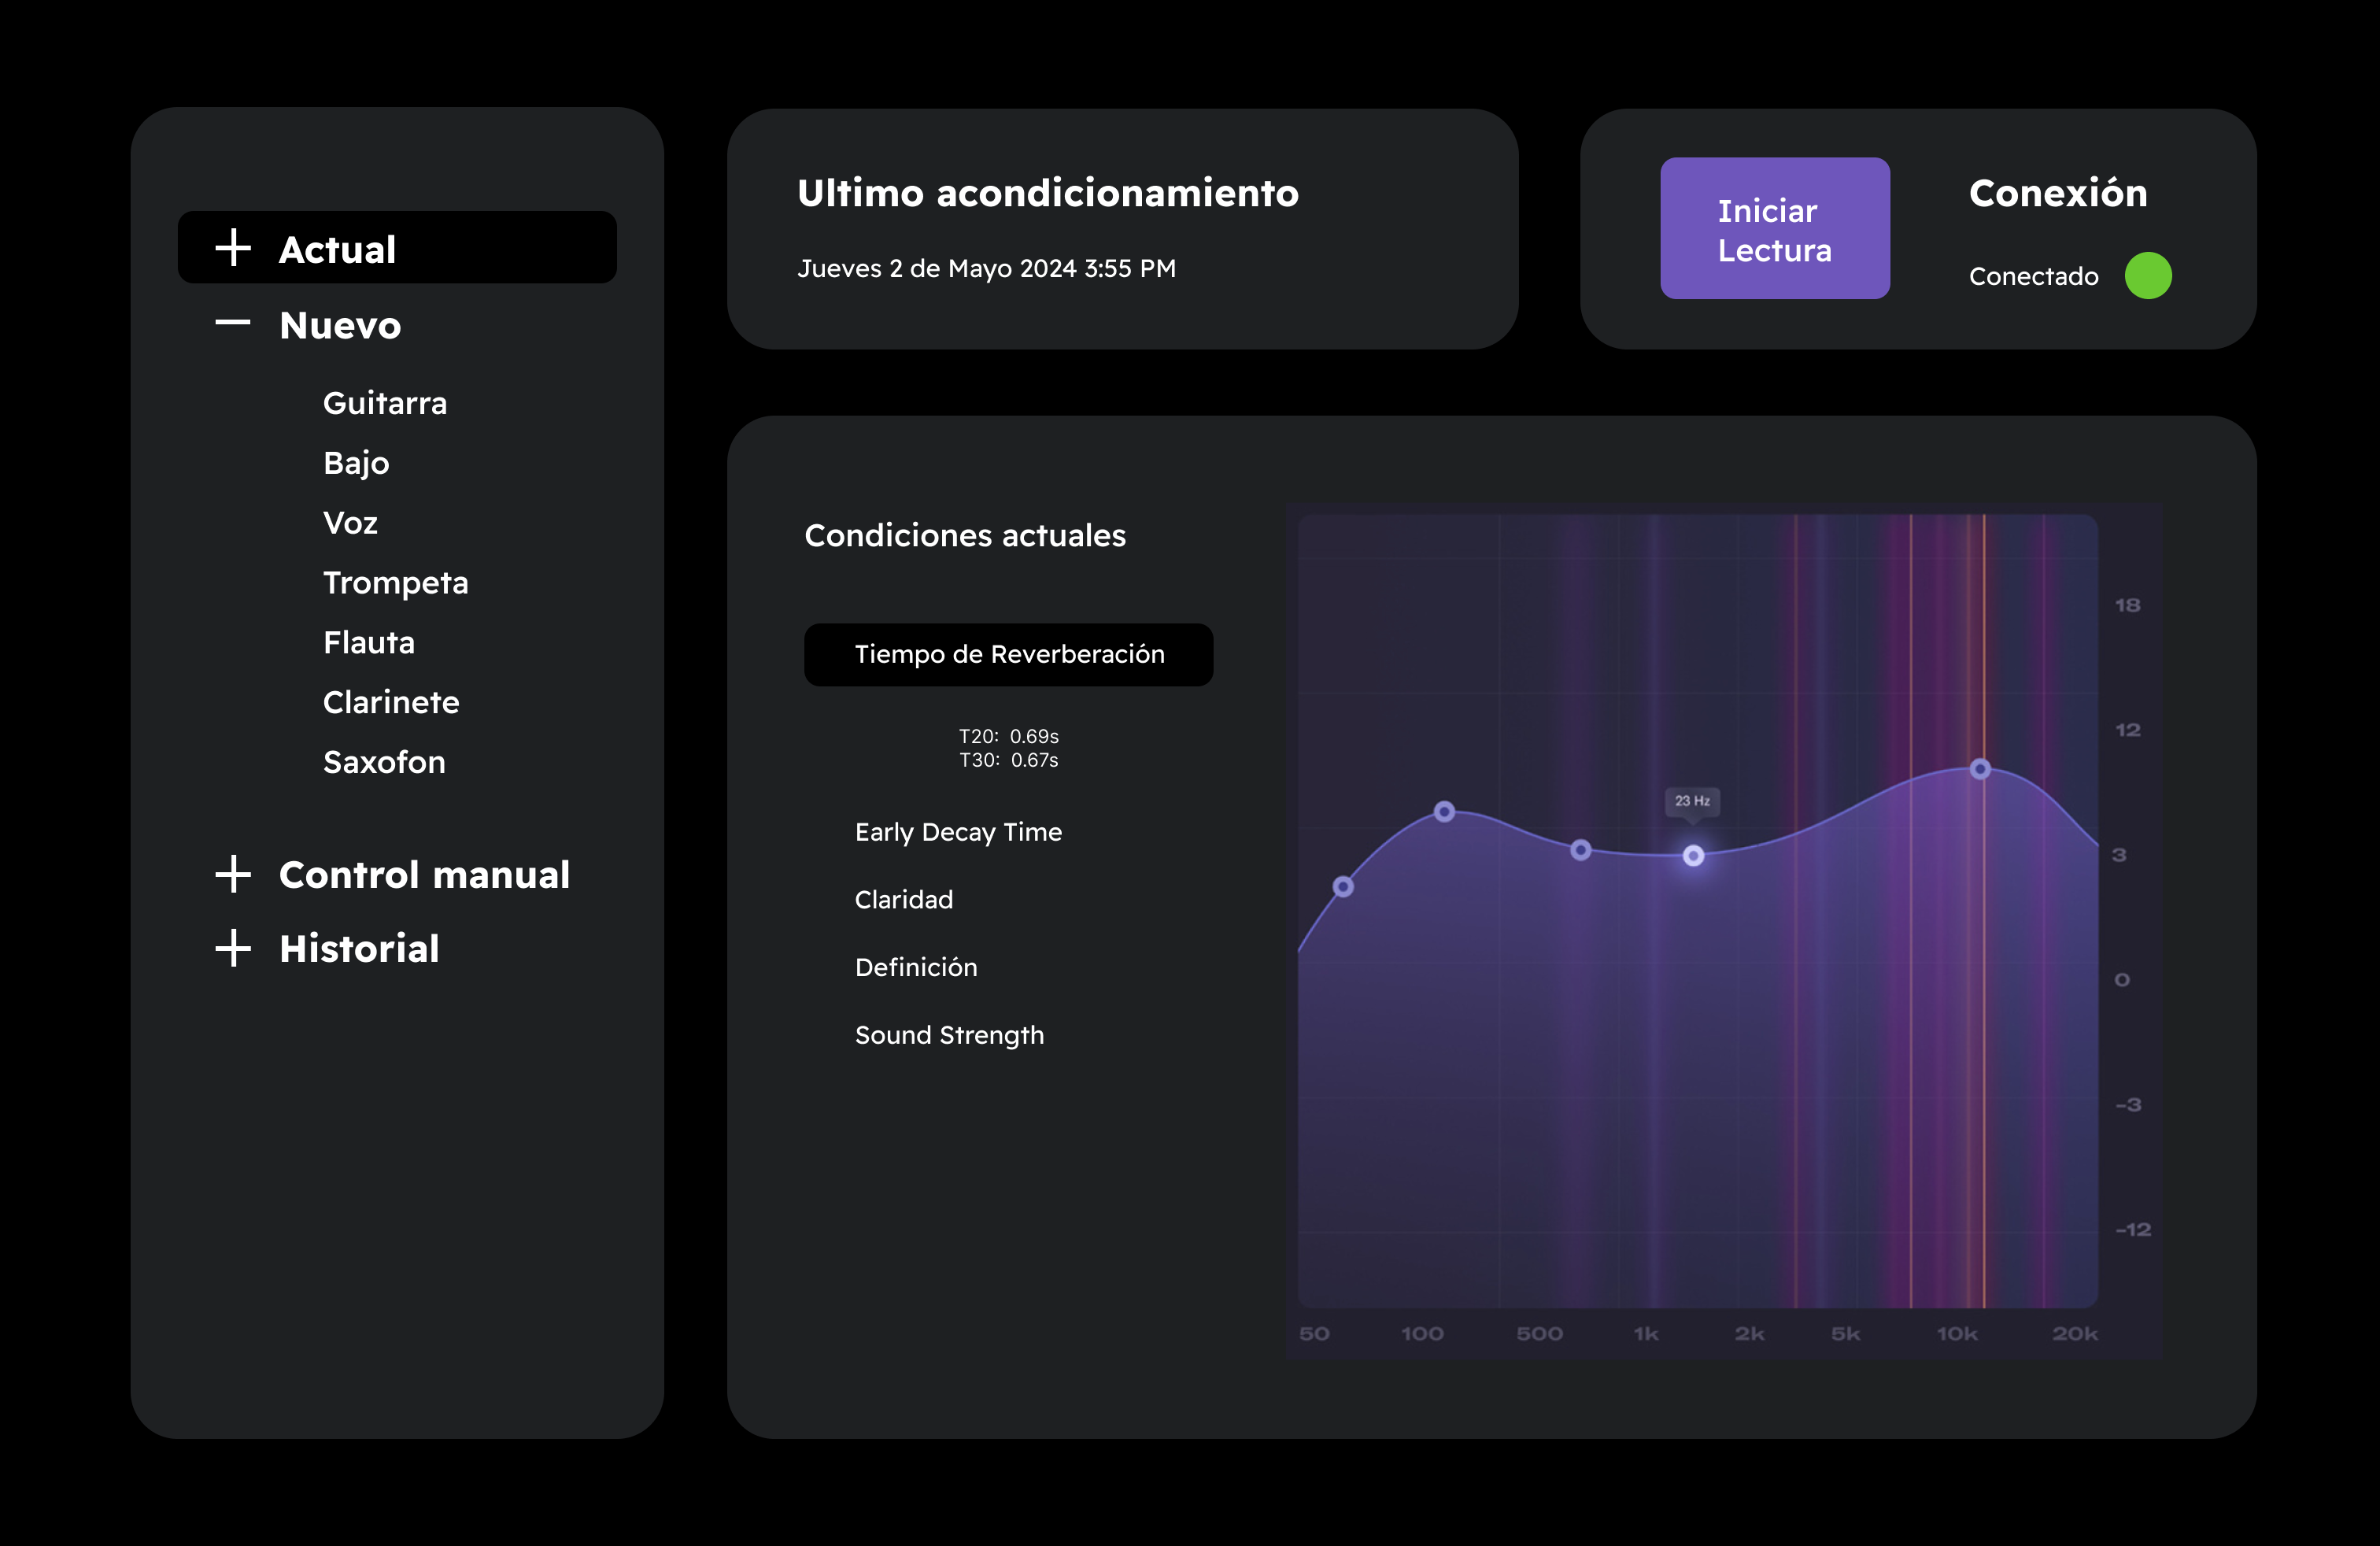
\includegraphics[width=\linewidth]{imagenes/Landing.png}
        \caption{\footnotesize Página de la acústica actual}
        \label{fig:pagina_home}
    \end{subfigure}
    \hfill
    \begin{subfigure}{0.45\textwidth}
        \centering
        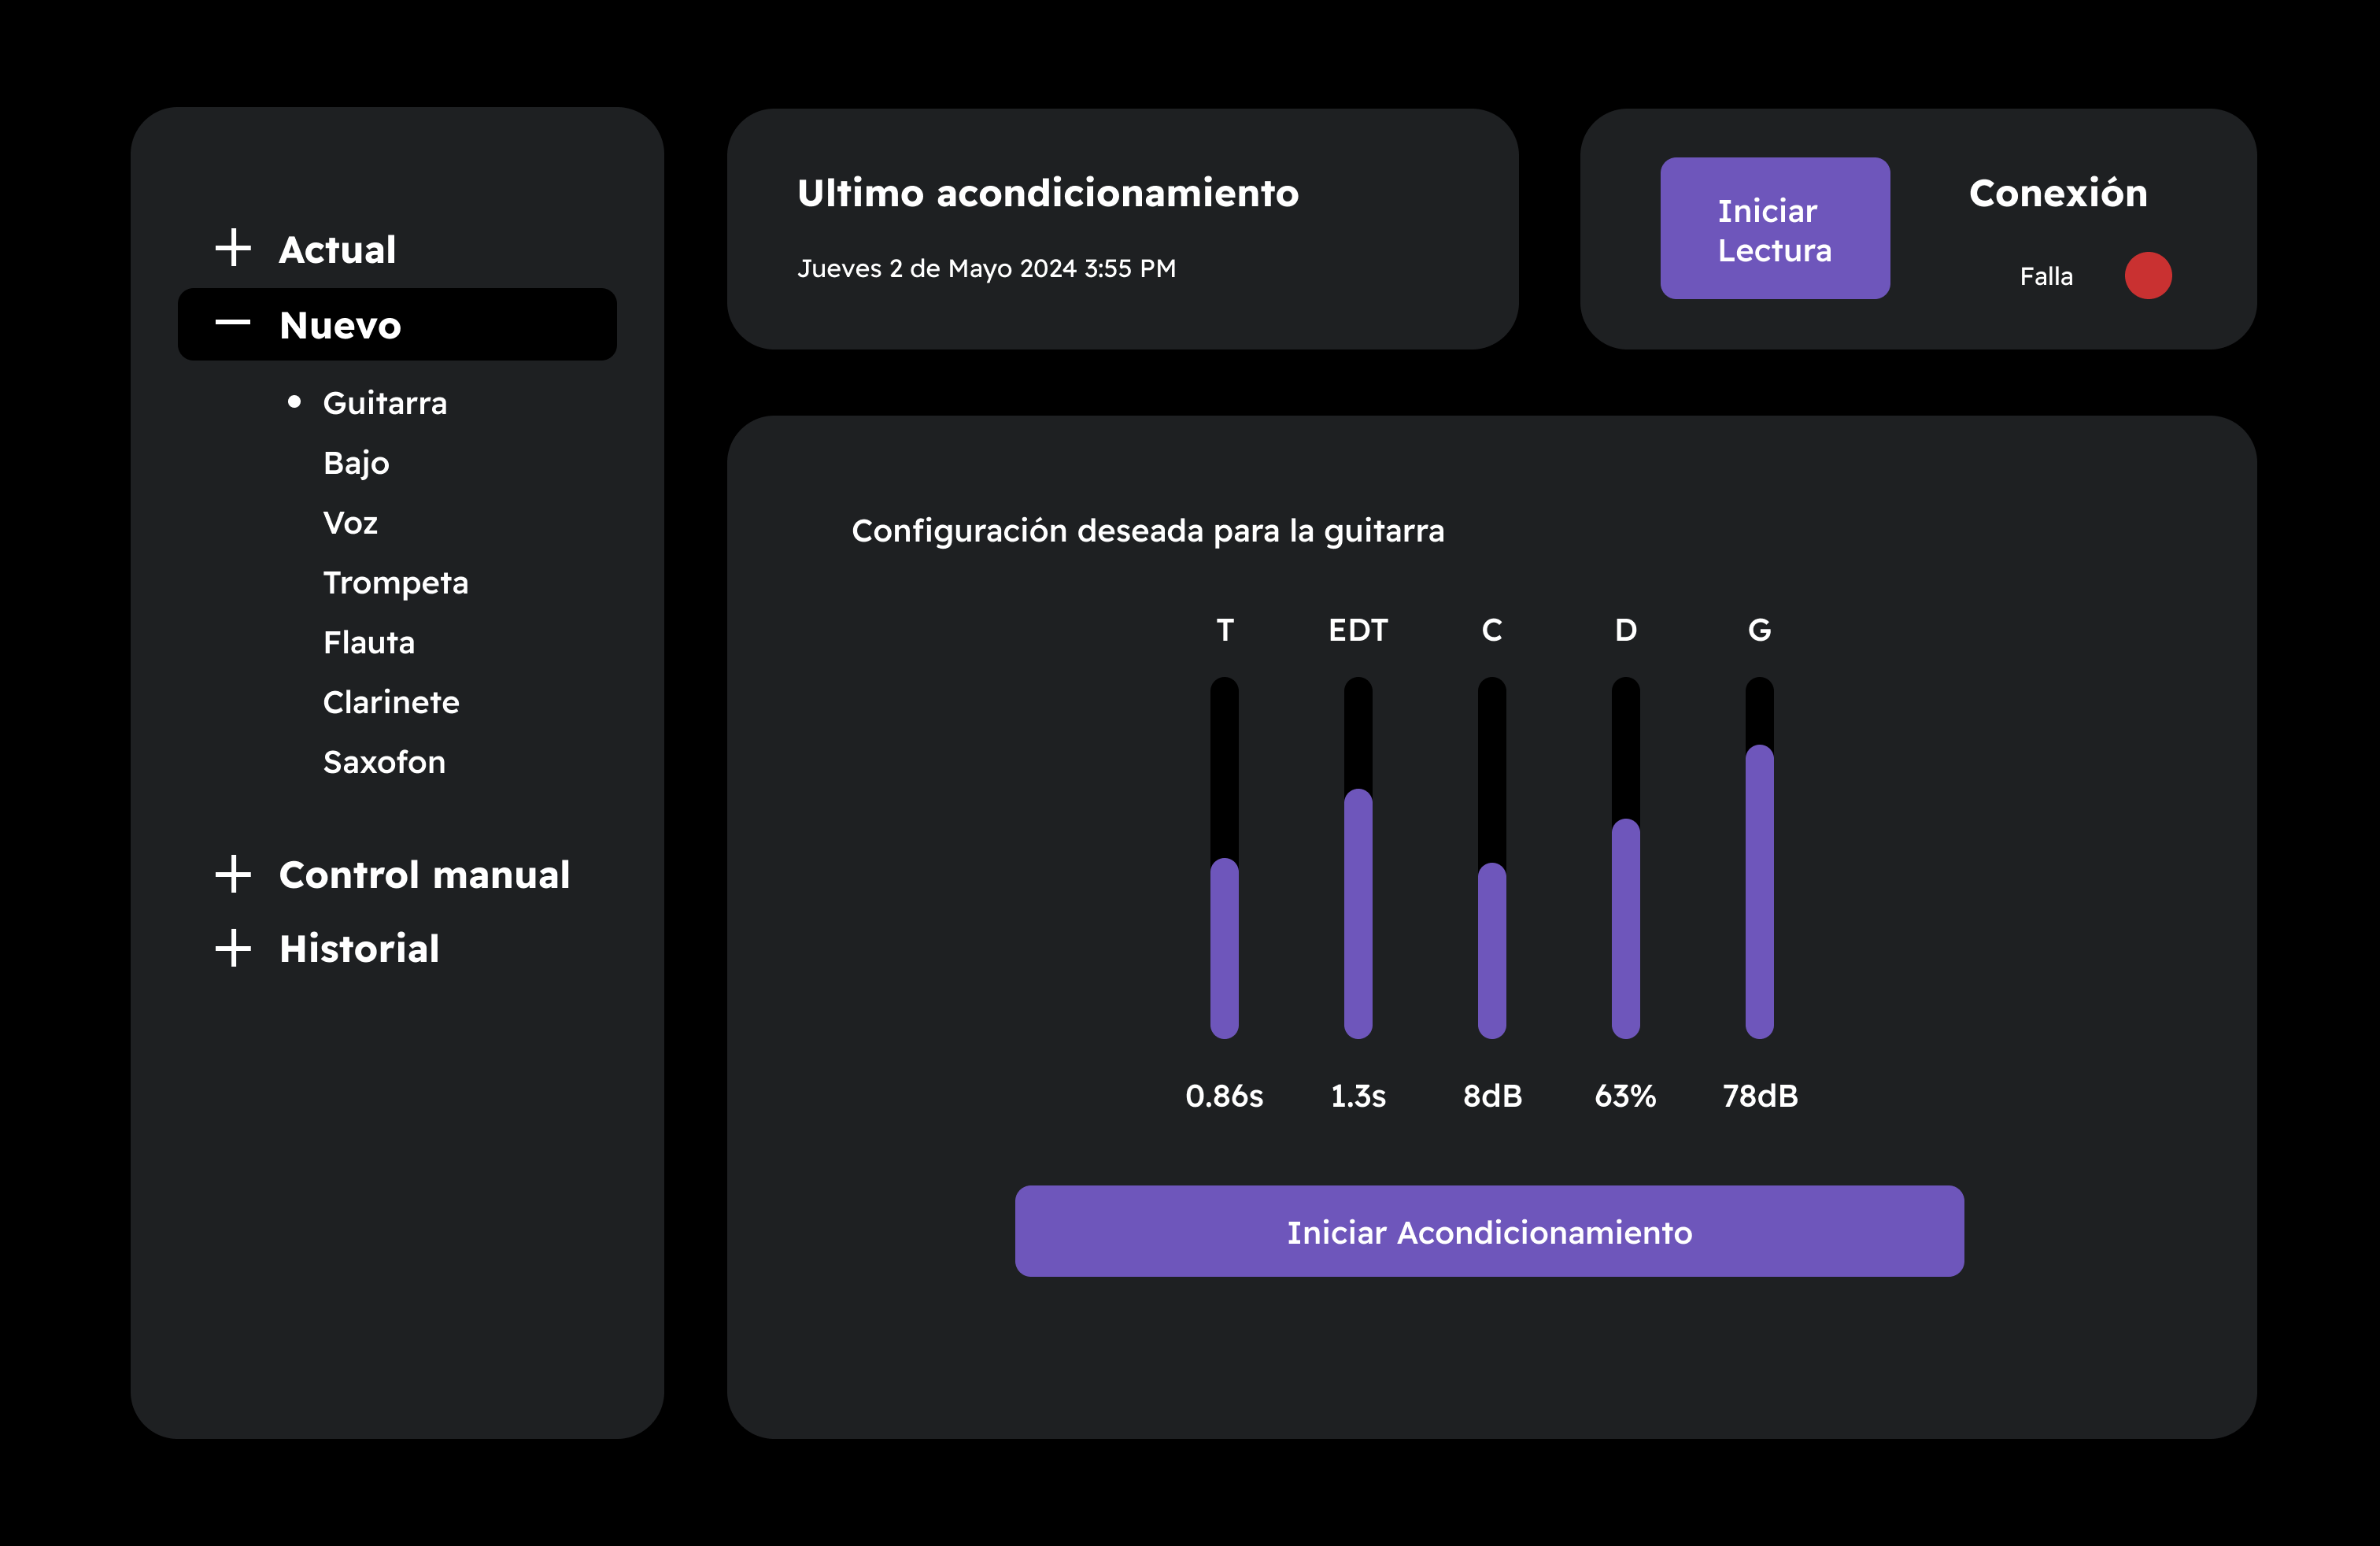
\includegraphics[width=\linewidth]{imagenes/Guitarra.png}
        \caption{\footnotesize Página generación de una nueva acústica}
        \label{fig:pagina_instrumento}
    \end{subfigure}
    \vskip\baselineskip
    \begin{subfigure}{0.45\textwidth}
        \centering
        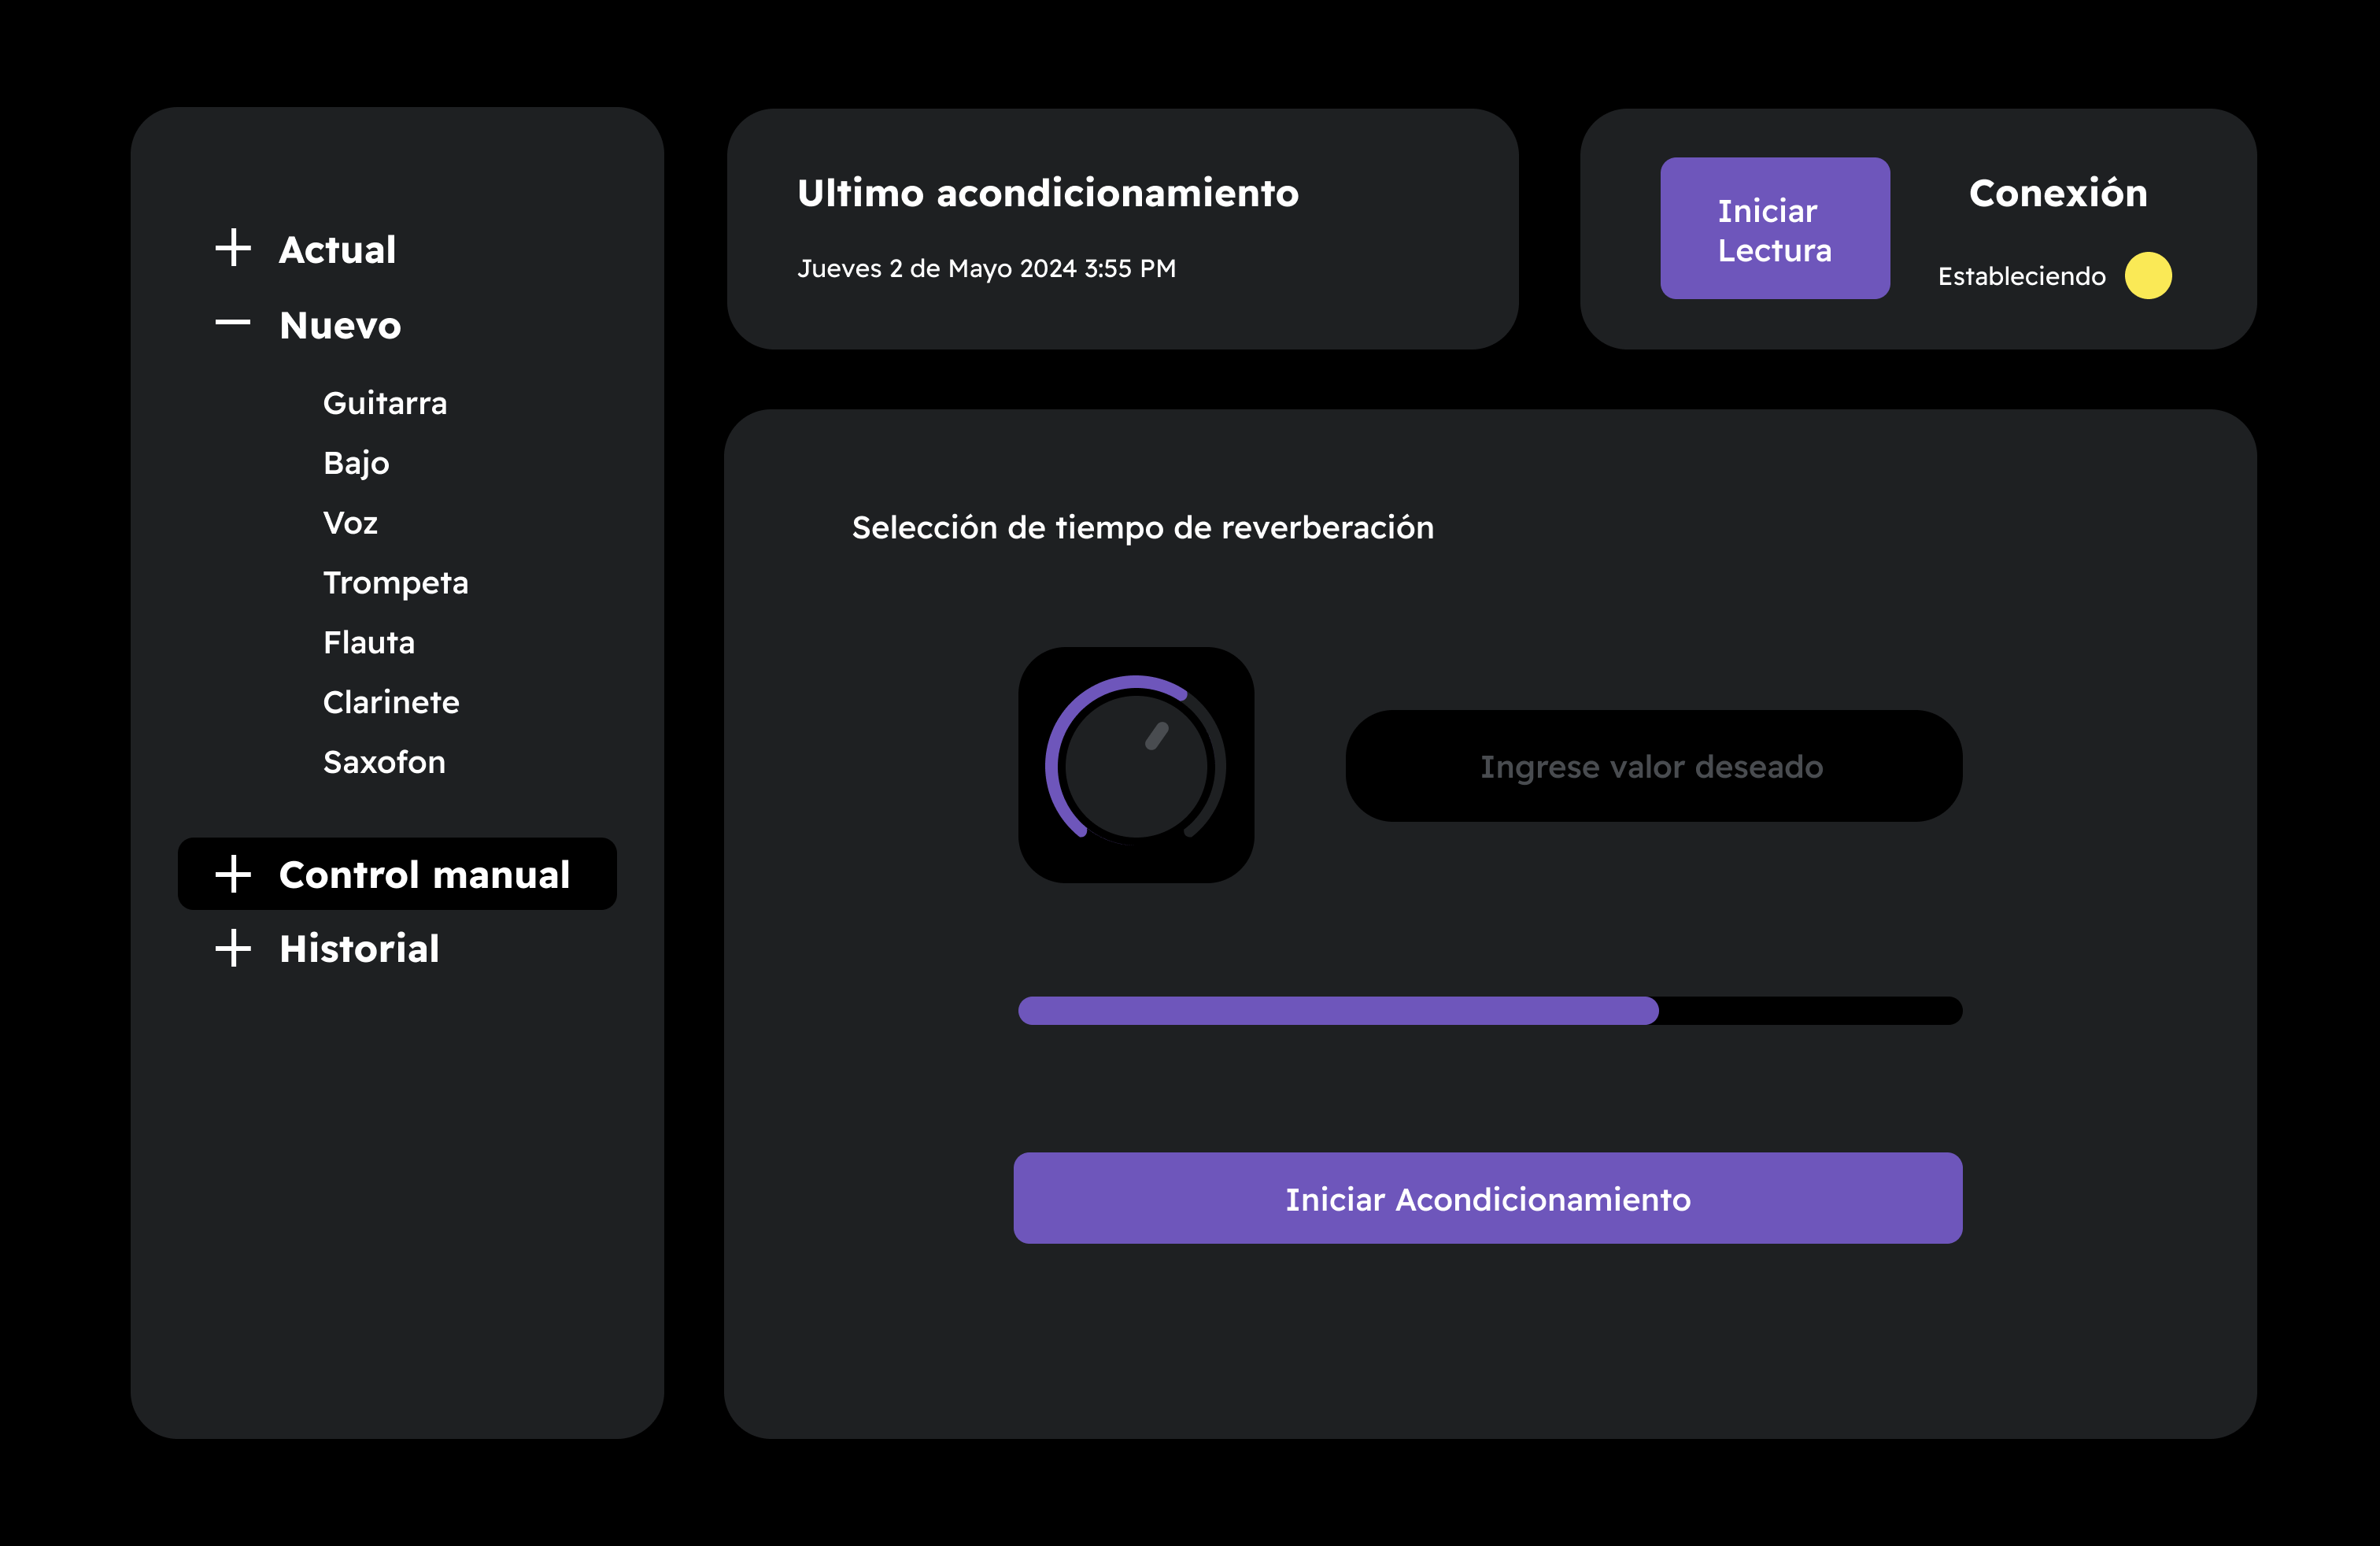
\includegraphics[width=\linewidth]{imagenes/Control Manual.png}
        \caption{\footnotesize Página de control manual}
        \label{fig:pagina_manual}
    \end{subfigure}
    \hfill
    \begin{subfigure}{0.45\textwidth}
        \centering
        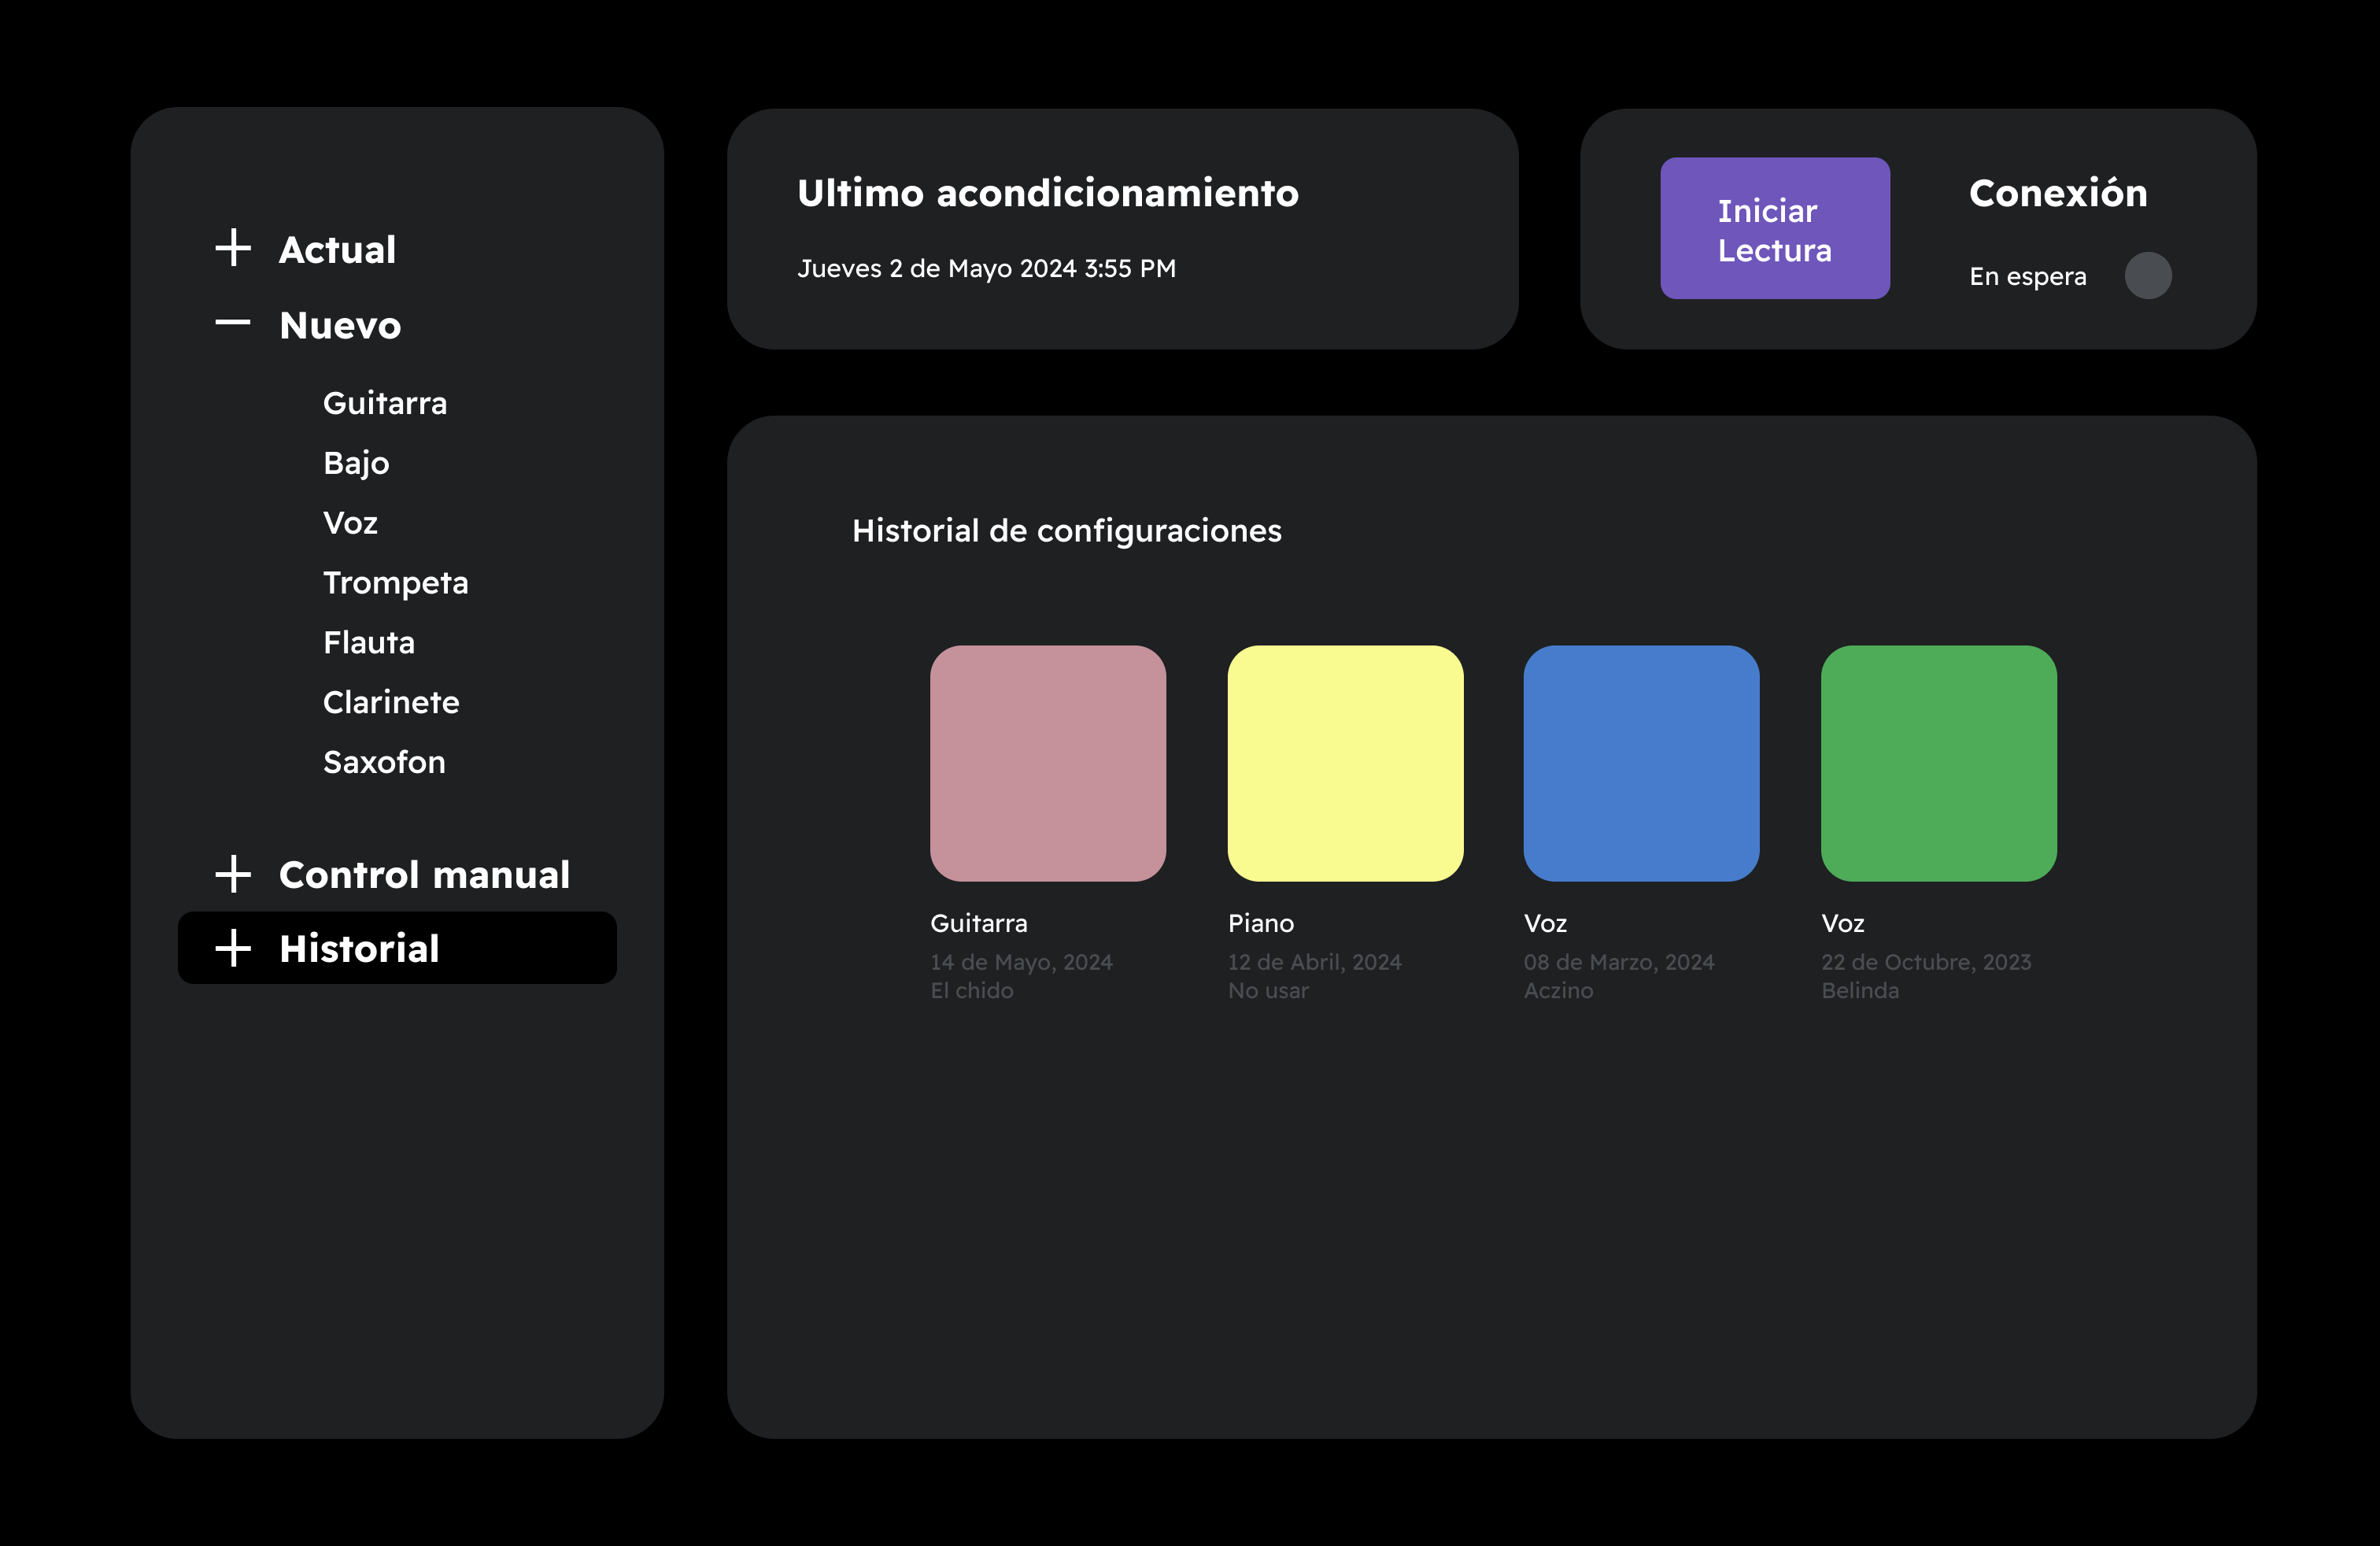
\includegraphics[width=\linewidth]{imagenes/Historial.png}
        \caption{\footnotesize Página del historial de configuraciones}
        \label{fig:pagina_historial}
    \end{subfigure}
    \caption{Vistas de la interfaz de usuario}
    \label{fig:vistas_interfaz}
\end{figure}
\FloatBarrier

Para el desarrollo ya de una manera técnica, hemos seleccionado tecnologías que nos permiten crear una aplicación robusta, eficiente y de fácil mantenimiento. La tecnología principal que utilizaremos es Electron, complementada con otras herramientas y marcos de trabajo. \\

\textbf{Electron}
\begin{itemize}[label={}, leftmargin=0pt]
    \item \textbf{Descripción:} Electron es un marco de trabajo para construir aplicaciones de escritorio utilizando tecnologías web HTML, CSS y JavaScript. Permite crear aplicaciones multiplataforma que pueden ejecutarse en Windows, macOS y Linux desde una única base de código.
    \item \textbf{Justificación:}
\end{itemize}

\begin{longtable}{|p{3cm}|p{10cm}|}
\hline
\textbf{Ventaja} & \textbf{Descripción} \\ \hline
Multiplataforma & Electron permite desarrollar una sola vez y desplegar en múltiples sistemas operativos, lo cual reduce el tiempo y los costos de desarrollo. \\ \hline
Tecnologías Web & Al utilizar HTML, CSS y JavaScript, podemos aprovechar la vasta cantidad de recursos, bibliotecas y herramientas disponibles en el ecosistema web. \\ \hline
Facilidad de Desarrollo & Electron simplifica la creación de interfaces de usuario atractivas y funcionales, lo que nos permite centrarnos en la lógica de negocio y la experiencia del usuario. \\ \hline
Comunidad y Soporte & Electron cuenta con una amplia comunidad de desarrolladores y una extensa documentación, facilitando la resolución de problemas y la implementación de características avanzadas. \\ \hline
\caption{Selección de marco de trabajo: Electron}
\end{longtable}

\textbf{React}
\begin{itemize}[label={}, leftmargin=0pt]
    \item \textbf{Descripción:} React es una biblioteca de JavaScript para construir interfaces de usuario. Permite crear componentes reutilizables que gestionan su propio estado, lo que facilita el desarrollo de aplicaciones dinámicas y responsivas.
    \item \textbf{Justificación:}
\end{itemize}

\begin{longtable}{|p{3cm}|p{10cm}|}
\hline
\textbf{Ventaja} & \textbf{Descripción} \\ \hline
Componentización & React permite dividir la interfaz de usuario en componentes reutilizables, lo que mejora la mantenibilidad y la escalabilidad del código. \\ \hline
Virtual DOM & React utiliza un DOM virtual para minimizar las actualizaciones en el DOM real, lo que mejora significativamente el rendimiento de la aplicación. \\ \hline
Comunidad y Ecosistema & React tiene una gran comunidad y un ecosistema robusto, con numerosas bibliotecas y herramientas que facilitan el desarrollo. \\ \hline
Aprendizaje y Uso & React es relativamente fácil de aprender y usar, con una sintaxis declarativa que simplifica la creación de interfaces de usuario complejas. \\ \hline
\caption{Selección de libreria de desarrollo principal: React}
\end{longtable}

\textbf{Redux}
\begin{itemize}[label={}, leftmargin=0pt]
    \item \textbf{Descripción:} Redux es una biblioteca de JavaScript para gestionar el estado de la aplicación de manera predecible. Comúnmente acompañada de React.
    \item \textbf{Justificación:}
\end{itemize}

\begin{longtable}{|p{3cm}|p{10cm}|}
\hline
\textbf{Ventaja} & \textbf{Descripción} \\ \hline
Manejabilidad del Estado & Redux proporciona una manera clara y predecible de gestionar el estado de la aplicación, facilitando la depuración y el mantenimiento del código. \\ \hline
Escalabilidad & Redux es adecuado para aplicaciones grandes y complejas donde el manejo del estado puede volverse complicado. \\ \hline
Ecosistema & Redux tiene un amplio ecosistema de herramientas y middleware que facilitan tareas comunes como la asincronía y la persistencia del estado. \\ \hline
\caption{Selección de gestor del estado: Redux}
\end{longtable}

\textbf{Styled Components}
\begin{itemize}[label={}, leftmargin=0pt]
    \item \textbf{Descripción:} Styled Components es una biblioteca de JavaScript que permite escribir estilos CSS dentro del código JavaScript utilizando una técnica llamada CSS-in-JS.
    \item \textbf{Justificación:}
\end{itemize}

\begin{longtable}{|p{3cm}|p{10cm}|}
\hline
\textbf{Ventaja} & \textbf{Descripción} \\ \hline
Encapsulación & Styled Components permite encapsular estilos dentro de los componentes, evitando conflictos de nombres y facilitando la mantenibilidad. \\ \hline
Dinamismo & Permite aplicar estilos dinámicos basados en props y estado, lo cual es ideal para interfaces de usuario interactivas. \\ \hline
Integración & Styled Components se integra perfectamente con React, permitiendo una experiencia de desarrollo fluida y consistente. \\ \hline
\caption{Selección de herramienta de estilizado: Styled Components}
\end{longtable}

\textbf{D3.js}
\begin{itemize}[label={}, leftmargin=0pt]
    \item \textbf{Descripción:} D3.js es una biblioteca de JavaScript para la visualización de datos que permite manipular documentos basados en datos.
    \item \textbf{Justificación:}
\end{itemize}

\begin{longtable}{|p{3cm}|p{10cm}|}
\hline
\textbf{Ventaja} & \textbf{Descripción} \\ \hline
Flexibilidad & D3.js permite crear visualizaciones de datos altamente personalizadas y interactivas. \\ \hline
Actualización Dinámica & Facilita la actualización dinámica de las visualizaciones en respuesta a cambios en los datos. \\ \hline
Comunidad y Recursos & D3.js cuenta con una amplia comunidad y una gran cantidad de recursos y ejemplos disponibles para aprender y resolver problemas. \\ \hline
\caption{Selección de herramienta de visualización: D3.js}
\end{longtable}

La combinación de Electron con React, Redux, Styled Components y D3.js funciona en sinergia de la siguiente manera: Electron para desarrollar la aplicación multiplataforma, React y Redux facilitan la construcción de la interfaz de usuario dinámica y gestionada de manera eficiente. Styled Components asegura que nuestros estilos sean modulares y mantenibles, y por ultimo D3.js nos permite ofrecer visualizaciones de datos ricas e interactivas.
Esta selección de tecnologías está cuidadosamente diseñada para satisfacer las necesidades de nuestro proyecto, garantizando tanto la experiencia de desarrollo, como el resultado para el usuario. \\

